%      Copyright (c) 2023 Cyril Huang, Gyoza Workshop
%      Permission is granted to copy, distribute and/or modify this document
%      under the terms of the GNU Free Documentation License, Version 1.1
%      or any later version published by the Free Software Foundation;
%      with the Invariant Sections being LIST THEIR TITLES, with the
%      Front-Cover Texts being LIST, and with the Back-Cover Texts being LIST.
%      A copy of the license is included in the section entitled "GNU
%      Free Documentation License".

\documentclass[a4paper,10pt,twoside]{book}

\usepackage{xeCJK}
\usepackage{fontspec}
\usepackage{wrapfig}
\usepackage{fancyhdr}
\usepackage{listings}
\usepackage{hyperref}
\usepackage{graphicx}
\usepackage[dvipsnames]{xcolor}
\usepackage{array}
\usepackage{makeidx}

\usepackage{layout}
\usepackage{pifont}
\usepackage{amsmath}
\usepackage{mflogo}
\usepackage{metalogo}
\usepackage{pgfplots}
\usepackage{tikz}

\usepackage[margin=2cm]{geometry}

\parindent=0pt
\pgfplotsset{compat=1.18,width=10cm}
\usetikzlibrary{patterns,snakes,ducks}

\setCJKmainfont{Noto Sans CJK TC}
\makeindex

\hypersetup{
  backref,
  unicode=true,
  bookmarks=true,
  pdfauthor=Cyril Huang,
  colorlinks=true,
  breaklinks=true,
  hyperfigures=true,
  pdfstartview=FitH,
  linkcolor=blue
}

\lstloadlanguages{bash,[ANSI]C,[gnu]make}
\lstset{basicstyle=\ttfamily\small,
    keywordstyle=\color{blue}\bfseries
}

\pagestyle{fancy}
\fancyhead[RO]{\small\bfseries\rightmark\ \ \thepage}
\lfoot{餃子出品必屬佳作}
\cfoot{}
\rfoot{}
 
\title{{\LaTeX} 基本寫作\thanks{大饅頭}}
\author{
  大頭\\
  cyril\_huang@gmx.com \\
  餃子出版社
  \and
  大雄\\
  shawn\_chiou@gmail.com \\
  餃子出版社
}

\begin{document}
  \maketitle
  \tableofcontents
  \input{tex.tex}
  \chapter{安裝與基本使用}
雖然現在有強大網頁版的 what you see is what you get 的 
\href{https://www.overleaf.com/}{overleaf},但自己本機裝比較隨心所欲。
有了上面的一些基本觀念,就可以安裝了, 過去有的 distribution 有
\begin{itemize}
 \item teTeX, 古老的 distro ,現在已經被 TeX Live 取代了,就把它想成 slackware 吧。
 \item TeX Live 目前最大的 \TeX distribution。所以我們就裝這個吧。
 \item MacTeX 蘋果用的。
 \item MiKTeX MS-Windows 用的。
\end{itemize}
當然其實在蘋果或MS Windows 也能用 \TeX Live,只是不知道為啥,大家都這樣推薦。
在目前 Linux 環境中,應該還是 \TeX Live 是主流,也簡單。

\section{從 Linux 上安裝}
網路上看很多人說安裝很難,對於 Linux 來說就一行命令就裝完了,真不知道難在哪裡
,真正難在怎麼裝的剛剛好你要的就好。
\\\\
debian/ubuntu
\begin{verbatim}
# apt install texlive-lang-chinese texlive-xetex
\end{verbatim}
redhat/centos/alma/rocky/fedora
\begin{verbatim}
# yum install texlive-collection-langchinese
\end{verbatim}
如果是 CentOS stream, Alma, Rocky 的 distro ,則在AppStream/ repository 下。
\\\\
以 debian / ubuntu 為例。可能碰到的錯誤跟 package
\begin{itemize}
\item texlive-lang-chinese 這個會裝一堆有的沒的包括 Big 5 碼的字型。還有相關
 macro,例如錯誤訊息找不到 ctexhook.sty

\begin{verbatim}
Building PDF for CJK languages fails with 'xeCJK.sty: File `ctexhook.sty' not found
\end{verbatim}

\item texlive-xetex 能處理很多 xetex 的相關 macro,然後奇怪的是 xeCJK 也在這裡。
\item texlive-luatex 能處理很多 luatex 的相關 macro。例如錯誤訊息

\begin{verbatim}
! LaTeX Error: File `luatexbase.sty' not found.
\end{verbatim}

\end{itemize}
裝起來後,debian 裡面的引擎在
\begin{verbatim}
/usr/share/texlive/texmf-dist/tex
\end{verbatim}
下面有
\begin{verbatim}
context  fontinst  generic  latex  latex-dev  
lualatex  luatex  plain  xelatex  xetex
\end{verbatim}
文件在
\begin{verbatim}
/usr/share/doc/texlive-doc
\end{verbatim}
macro 的用法可以在下面找到。使用 distribution 收集的文件閱讀工具 texdoc 來搜尋與閱讀
\begin{verbatim}
$ texdoc -l luatexja
$ texdoc -s ams
\end{verbatim}
不過很多想看的都沒有找到,可能沒有裝 package,所以可能直接 google texdoc amsmath,
texdoc listings 等等的直接幫你找到 CTAN 的文章比較快。新的 
\href{https://texdoc.org}{texdoc 網站}也有搜尋整個 tex 文件的能力。

\section{中文使用}
先來看看我們有什麼字型可以用。fc-list 命令第二欄位就是字型名稱,
可以在 \LaTeX{} 設定中使用的。
\begin{verbatim}
$ fc-list 
\end{verbatim}
grep traditional chinese or taiwan
\begin{scriptsize}
\begin{verbatim}
$ fc-list | grep '\(TC\|TW\)'
$ fc-list :lang=zh-tw
/usr/share/fonts/truetype/arphic/uming.ttc: AR PL UMing TW MBE:style=Light
/usr/share/fonts/opentype/noto/NotoSerifCJK-Bold.ttc: Noto Serif CJK TC:style=Bold
/usr/share/fonts/opentype/noto/NotoSansCJK-Black.ttc: Noto Sans CJK TC,Noto Sans CJK TC Black:style=Black,Regular
/usr/share/fonts/opentype/noto/NotoSansCJK-Regular.ttc: Noto Sans CJK TC:style=Regular
/usr/share/fonts/opentype/noto/NotoSerifCJK-Regular.ttc: Noto Serif CJK TC:style=Regular
/usr/share/fonts/opentype/noto/NotoSerifCJK-ExtraLight.ttc: Noto Serif CJK TC,Noto Serif CJK TC ExtraLight:style=ExtraLight,Regular
/usr/share/fonts/opentype/noto/NotoSansCJK-DemiLight.ttc: Noto Sans CJK TC,Noto Sans CJK TC DemiLight:style=DemiLight,Regular
/usr/share/fonts/opentype/noto/NotoSansCJK-Medium.ttc: Noto Sans CJK TC,Noto Sans CJK TC Medium:style=Medium,Regular
/usr/share/fonts/opentype/noto/NotoSerifCJK-Black.ttc: Noto Serif CJK TC,Noto Serif CJK TC Black:style=Black,Regular
/usr/share/fonts/opentype/noto/NotoSansCJK-Bold.ttc: Noto Sans Mono CJK TC:style=Bold
/usr/share/fonts/opentype/noto/NotoSerifCJK-Medium.ttc: Noto Serif CJK TC,Noto Serif CJK TC Medium:style=Medium,Regular
/usr/share/fonts/truetype/arphic/uming.ttc: AR PL UMing TW:style=Light
/usr/share/fonts/opentype/noto/NotoSerifCJK-SemiBold.ttc: Noto Serif CJK TC,Noto Serif CJK TC SemiBold:style=SemiBold,Regular
/usr/share/fonts/opentype/noto/NotoSansCJK-Regular.ttc: Noto Sans Mono CJK TC:style=Regular
/usr/share/fonts/opentype/noto/NotoSerifCJK-Light.ttc: Noto Serif CJK TC,Noto Serif CJK TC Light:style=Light,Regular
/usr/share/fonts/opentype/noto/NotoSansCJK-Thin.ttc: Noto Sans CJK TC,Noto Sans CJK TC Thin:style=Thin,Regular
/usr/share/fonts/opentype/noto/NotoSansCJK-Bold.ttc: Noto Sans CJK TC:style=Bold
/usr/share/fonts/opentype/noto/NotoSansCJK-Light.ttc: Noto Sans CJK TC,Noto Sans CJK TC Light:style=Light,Regular
\end{verbatim}
\end{scriptsize}
其中第二欄位的名字就是拿來設定字型用的,有逗號表示多種別名。
\\\\
使用古老的 pdftex 引擎也能處理 unicode ,
但選擇能直接處理 unicode ttf/otf 的 lualatex 或 xelatex 引擎與工具。
\\\\
lualatex 範例:

\begin{verbatim}
\documentclass[a4paper,10pt]{book}
\usepackage{luatexja-fontspec}
\setmainjfont{Noto Serif CJK TC}

\begin{document}
\chapter{第一章}
大頭
  \section{第一節}
  小頭
\end{document}
\end{verbatim}

xelatex 範例:

\begin{verbatim}
\documentclass[a4paper,10pt]{book}
\usepackage{xeCJK}
\setCJKmainfont{Noto Serif CJK TC}

\begin{document}
\chapter{第一章}
大頭
  \section{第一節}
  小頭
\end{document}
\end{verbatim}

用標準英文 macro 排點簡單的也可以,
但一些嚴格複雜的排版規矩是會失敗的。

\begin{verbatim}
\documentclass[a4paper,10pt]{book}
\usepackage{fontspec}
\setmainfont{Noto Serif CJK TC}

\begin{document}

\chapter{第一章}
大頭大頭下雨不愁,人家有傘你有大頭。
  \section{第一節}
  小頭銳面難以哉。鄭燮寄弟墨書:「其不發達者,鄉里作惡,小頭銳面,更不可當。」
  頭小而臉尖。形容人刁頑刻薄。又作「小頭小臉」。

\end{document}
\end{verbatim}
lualatex 中文社群決定不開發新的 package ,沿用日本的 luatexja 就好,因為
漢字處理兩者是一樣的,即使 CJKV 這四個漢字圈的韓國越南大概也不用漢字了。
\\\\
命令差別在於設定字型新命令,setmainjfont, setCJKmainfont, 與標準英文的
setmainfont。之所以要使用特別 package 在於排版規矩,漢字與英文在斷行,
間隔,空白,寬度計算上有些不同,又或者漢字能直排等等。如果不是很在意排
版效果,用全英文的命令都可以。
\\\\
命令產生 pdf 檔

\begin{verbatim}
$ xelatex test.tex
$ lualtex test.tex
\end{verbatim}

如果有錯誤發生,應該是某相依 macro 沒有裝起來,去 google 看要裝什麼名字,
在系統中安裝。過去可能會先產生 dvi 檔,再由 dvi 轉成各種輸出,或者將 latex 
轉成 html, opendoc 等等,不過現在網路速度很快,使用 pdf 在線閱讀也沒問題,
所以也不再做這些輸出,有興趣的就自己玩其他的工具。
\\\\
有的例子會用 \verb=\usepackage{CJK}= 套件,這個套件是舊的 pdftex 使用的,
所以它的目錄編排方式好像還是以前 teTeX 的 /usr/share/texmf/tex 而不是
/usr/share/texlive/texmf-dist, 它也有 UTF8 編碼, 如果真有 Big5, 
GB, JIS 編碼舊文件要處理,也可以用這套件,只是 pdftex 它字型使用
必須是相關 tfm/map 已經建立,所以若是建立不完全則無法使用。
而設定名字必須是從 fd 檔裡面找到真正字型名稱用在 CJK package 裡面。
我就是從 /usr/share/texlive 跟 /usr/share/texmf 下面搜尋 fd 檔,
然後去看名稱,因此用 pdflatex 除非自己懂造新字型的,不然是很受限
於 distro 給你的字型。
\\\\
pdflatex 範例
\begin{verbatim}
\documentclass[a4paper,10pt]{book}
\usepackage{CJK}

\begin{document}
\begin{CJK}{UTF8}{bkai}
\chapter{第一章}
大頭大頭下雨不愁,人家有傘你有大頭。
  \section{第一節}
  小頭銳面難以哉。鄭燮寄弟墨書:「其不發達者,鄉里作惡,小頭銳面,更不可當。」
  頭小而臉尖。形容人刁頑刻薄。又作「小頭小臉」。

\end{CJK}
\end{document}
\end{verbatim}
使用命令為 
\begin{verbatim}
$ pdflatex test.tex
\end{verbatim}
這個 bkai 名字是 fd 檔案裡面的,這是 Big 5 楷書,只是用 pdflatex 引擎,
可以轉換 Big 5 到 UTF8。 最後編譯如果出錯,都會有個 xxx.log 檔,裡面會有
整個編譯總結,錯誤訊息都在裡面。

\section{進階安裝}
其實像我安裝 Linux 時,我都是裝我需要的東西就好,有些大 package 的安裝,
裝了一大堆亂七八糟的東西,但要做到只安裝有需要的,就必須對整個系統有粗淺的了
解才有可能。
\\\\
texlive 最基本會包 plain \TeX, pdftex, luatex
\subsection{最小安裝 - deb package}
從目前 debian/ubuntu 的 package 來看
\begin{itemize}
\item texlive-base 只有包含引擎 tex, pdftex, luatex
\item texlive-binaries dvi, metafont, metapost, ps 等處理程式,然後還有 xetex。
\item texlive-latex-base 包含 latex, pdflatex, lualatex
\item texlive-xetex 才會包含 xelatex 與相關工具。
\item texlive-luatex 才會包含相關 macro 。
\end{itemize}
不知道為什麼目前 xetex 是被特別對待的,也就是 luatex 是自動在 texlive-base,
但 xetex 卻是在 texlive-binaries,總之,base 與 binaries 是引擎與基本工具。
\\\\
中日韓套件
\begin{itemize}
\item texlive-lang-xxxx 這些才是新的 \XeTeX 需要的。
  \begin{itemize}
  \item texlive-lang-chinese 是真正有一些中文處理 sty ,fd 檔,與文鼎
   truetype 字型,會把 texlive-lang-cjk 這些亂七八糟的全裝起來。
   這些 package 實在分類裝的亂七八糟的。
  \item texlive-lang-cjk 一些 mapping 檔。
  \item texlive-xetex 裡面才有真正 xeCJK macro
  \end{itemize}
\item latex-cjk-xxxx 都是舊的古老的工具
  \begin{itemize}
  \item latex-cjk-chinese 是真正有如 bg5latex,包含big5, gb 碼等工具。
        如果改用新的 unicode {\XeTeX} luatex 引擎,這些是可以不要裝的。
  \item latex-cjk-common 是用在 pdftex 上的 macro
  \end{itemize}
\end{itemize}
字型在以前是系統跟 \TeX 系統是分開的,要分別為他們兩個需求建立特別系統需要檔案,
現在 {\XeTeX} luatex 能統一用所有的,系統上就應該是免費的 google No Tofu 
計畫裡面的 opentype ,同樣 latex-cjk-xxx 的是舊的特有 \TeX 需求檔案,font-xxx
是系統字型檔。
\begin{itemize}
\item fonts-noto-cjk google 的開源 No Tofu 思源字體。系統上 opentype 字體。
\item fonts-arphic-xxx 文鼎 truetype 字型,有人改了原本type1 big5 編碼成為 
truetype unicode 編碼給大家用。
\item fonts-wqy-xxx 文泉驛字型。
\item latex-cjk-chinese-arphic-xxx 這是舊的文鼎 type 1 字型。
有 tfm, fd 與 pfb 檔建好了,所以以前都是用這個。這還是可以給 xetex/luatex
繼續用,只不過字型命名方式不一樣。
\end{itemize}
pdftex 引擎比較麻煩,在 TEXMFHOME 目錄下搜尋 fd 檔,字型名字在裡面
,TEXMFHOME 應該在 /usr/share/texlive 與 /usr/share/texmf。
\\\\
所以真正安裝
\begin{itemize}
\item xelatex 這要裝 texlive-xetex, texlive-lang-chinese,
但它的 dependancy 太多。
\item lualatex 這要裝 texlive-luatex
\item fonts 喜歡的裝就好了。
\end{itemize}
rpm 形式的反而比 deb 的複雜很多。就先不管它了

\subsection{最小安裝 - 從CTAN}
如果沒有 root 權限,或不想裝 Linux 系統 package ,那麼就自己從 CTAN 抓 texlive
來,只是這我裝起來也要1G,也蠻大的。
\begin{enumerate}
\item \href {http://mirror.ctan.org/systems/texlive/tlnet/install-tl-unx.tar.gz}{CTAN 下載}
\item 執行 ./install-tl
\item 調整選項,按 S 選 c ,small scheme, 這個會裝 xetex 引擎。
\item 繼續調整其他,按 D 像是 TEXDIR TEXMFHOME 目錄。
\item 裝完後,要多增加 PATH, MANPATH, INFOPATH,就可以用了。
\end{enumerate}
\begin{center}
\includegraphics[width=\textwidth,height=0.6\textwidth]{images/texlive.png}
\end{center}
試看看最基本的命令
\begin{verbatim}
$ tex '\empty Hello world!\bye'
$ pdftex '\empty Hello world!\bye'
\end{verbatim}
像 python 用 pip ,perl 用 cpan,texlive 也有工具來管理 package,
而且也是遠端跟 CTAN 直接溝通的管理, 使用 tlmgr 來管理 macro。
package 管理只有幾件重要事情
\begin{itemize}
\item 遠端 repository 是誰?內定是 CTAN。
\item 本地端要裝在哪裡? 這應該在 TEXMFHOME 下。
\item 現在裝了什麼?
\item 如何安裝新的與移除不要的?
\item package 資訊與 package 裡面有什麼檔案?
\item 如何升級?
\item 怎麼移除全部安裝?
\end{itemize}
看看裝了什麼 package
\begin{verbatim}
$ tlmgr list
\end{verbatim}
安裝移除。我們是要裝 xecjk 的,所以 remove 只是命令。
\begin{verbatim}
$ tlmgr install xecjk
$ tlmgr remove xecjk
\end{verbatim}
package 的資訊
\begin{verbatim}
$ tlmgr info xecjk
$ tlmgr info --list xecjk
\end{verbatim}
尋找
\begin{verbatim}
$ tlmgr search --global --file cfr-lm.sty
$ tlmgr list | grep ducks 用 search 有的是找不到,用 grep 比較好
\end{verbatim}
升級
\begin{verbatim}
$ tlmgr update --list
$ tlmgr update --all
\end{verbatim}
設定原本的內定值,例如換掉遠端 repository 的位址
\begin{verbatim}
$ tlmgr option repsoitory https://mirror.ctan.org/systems/texlive/tlnet
$ tlmgr paper letter
\end{verbatim}
不爽玩了,整個毀掉
\begin{verbatim}
$ tlmgr uninstall
\end{verbatim}

\subsection{字型}
除了 Linux package 上有的,也可自行去抓 ttf 或者 otf 檔。如果沒有權限裝在系統
上,可以下載到 
\begin{verbatim}
\$HOME/.local/share/fonts 
或者舊的
\$HOME/.fonts 下
\end{verbatim}
然後用
\begin{verbatim}
$ mkfontscale
$ mkfontdir
$ fc-list
\end{verbatim}
製作向量字型 index 。
\\\\
下載中文字型,不過這很多在系統 package 上也是有啦,現在主要用 google
Adobe 合作的 opensource 思源字體,Noto 字體,不過用系統裝的跟下載的名字
有時會不同,不知為啥,我用 debian 系統package裝的是
Noto Sans CJK TC 但自己下載的變成 Noto Sans TC,所以這個名字要自己根據
fc-list 看到得來。不過台灣官方的全字庫跟教育部標準應該蒐集字是最齊全的,有些
冷門字,或許他們才有。
\begin{enumerate}
\item \href{https://data.gov.tw/dataset/5961}{數位發展部的全字庫宋體與楷書}
\item \href{https://language.moe.gov.tw/result.aspx?classify_sn=23&subclassify_sn=436}{教育部國字標準字體-宋楷隸}
\item \href{https://source.typekit.com/source-han-serif}{Adobe 的開源opentype思源字型}
\item \href{https://fonts.google.com/}{Google 的思源字體下載}
\item \href{https://github.com/fontworks-fonts}{日本Fontworks Inc的七款日文字體}
\item \href{https://github.com/googlefonts/kosugi-maru}{日本-日文小杉丸體}
\item \href{https://github.com/ichitenfont/I.Ming}{一點明體-修改日本 ichiten 的明體}
\item \href{https://sites.google.com/view/jtfoundry/zh-tw}{台北黑體-翰字鑄造公司改造思源適合印刷字型}
\item \href{https://github.com/ButTaiwan/iansui}{芫荽字體-新增改造fontworks 的klee而來}
\item \href{https://github.com/justfont/open-huninn-font}{粉圓體-新增改造小杉丸來}
\item \href{https://github.com/l10n-tw/cwtex-q-fonts}{cwTeX truetype}
\item \href{https://code.google.com/archive/p/wangfonts/}{王漢宗老師的48套字型}
\end{enumerate}
由於xelatex 是走系統字型, 系統字型套件是 fontconfig, 字型放在 /usr/share/fonts
\$HOME/.local/share/fonts 或者 \$HOME/.fonts ,設定在 /etc/fonts,
/usr/share/fontconfig,\$HOME/.config/fontconfig \$HOME/.fontconfig 下的
fonts.conf 與裡面的 conf.d 目 錄。 所以如果是手動用 install-tl 裝 texlive 的,
那要把 texlive 字型告訴 fc 進到系統字型設定中。 在安裝目錄下的
\begin{verbatim}
./texmf-var/fonts/conf/texlive-fontconfig.conf
\end{verbatim}
已經有 texlive 給 fontconfig 用的 conf 檔,是根據當初給的 TEXDIR TEXMFHOME
目錄建立的。因此只要 symlink 這檔案到
\begin{verbatim}
/etc/fonts/conf.d/90-texlive-fontconfig.conf
或
~/.config/fontconfig/confd.d/90-texlive-fontconfig.conf
或
~/.fonts.conf.d/90-texlive-fontconfig.conf
\end{verbatim}
就可以 fc-list 看到他們,
\\\\
texlive 在他目錄下 texmf-dist/fonts/type1 裡面 cjk 帶有 arphic 繁體字字型,
是文鼎以前 open 的字型,texmf-dist/fonts/misc/cns 裡面有 CNS 國家中央標準局
的 bitmap 字型,這好像是現在數位發展部負責了。但 arphic 是 Big5,而 cns 是
CNS 碼還是 bitmap,所以我想應該沒人會用了,不知道為啥安裝 cjk 套件還裝這些。
當用
\begin{verbatim}
tlmgr list | grep arphic
\end{verbatim}
還會發現有 arphic-ttf ,但也是 Big 5 的。 如果沒有抓其他的字體,光想用
texlive 原裝內定的下載使用 unicode 正體中文,
\begin{itemize}
  \item 使用傳統 pdflatex 用 \verb=\usepackage{CJK}= 與
    \verb=begin{CJK}{UTF8}{bkai}=
  \item 要不就是檔案是 input Big 5 使用 xelatex,lualatex 的 arphic-ttf
  \item fontspec 會自己抓 input encode (character code set) 跟 font encode 
    (font code set) 但這個要有 def 檔定義,目前好像沒有 big5<->utf8 定義檔
    給 xelatex 用。
  \item 自己用arphic Big5 生成 arphic unicode ttf/otf,不過這對新手有點煩。
    這乾脆下載自己的ttf 還比較快。debian 裡面有 arphic utf8 的 ttf package
    但這已經不是 texlive 原裝的了。
\end{itemize}
type1 基本上已經很老舊,對新手不是很好用,只是不知道為啥 Texlive 裡面
有中國大陸的 fando 簡體中文字型, 沒有 unicode 正體中文 ttf/otf,
連 noto 中文 TC 字型也沒有收錄。

  \chapter{\LaTeX{} 與 packages 的使用}
參考資料講解可以從
\begin{itemize}
  \item \href{https://en.wikibooks.org/wiki/LaTeX}{wikibook \LaTeX{}}
  \item \href{https://en.wikibooks.org/wiki/TeX}{wikibook \TeX{}}
  \item \href{https://latexref.xyz}{非官方 \LaTeX{} reference}
  \item \href{https://texdoc.org}{texdoc 網站}
  \item \href{https://www.tug.org/texlive/devsrc/Master/doc.html}
    {TeXLive 收集的 package 文件}
  \item \href{https://www.overleaf.com/learn}{overleaf 學習網站}
\end{itemize}
都是標準 package ,剩下的都是屬於更細微的調整,所以最後只是去找 package
的詳細 reference 說明使用而已,而如果用 CTAN script 自己安裝的,用 tlmgr
裝 package 時,也都會把 pdf 文件安裝進來,在 TEXDIR 下搜尋 pdf 檔都能找到。
\\\\
{\LaTeX} 如果是多檔使用,可以用
\begin{verbatim}
\begin{docuemnt}
\include{chapter1}
 或者
\input{chapter1.tex}
\end{document}
\end{verbatim}
include 一定要是 .tex 副檔名,且不可寫副檔名,
input 則可以使用別的副檔名,副檔名可寫可不寫。

\section{書籍排版元素}
除了基本的章節段落 \verb=\chapter{} \section{} \subsection{} \paragraph{}=,
強迫分行使用兩個反斜線,\verb=\\=,所以空一行就要 \verb=\\\\= ,或者用
\verb=\\[1cm]= 指定換行空白大小。光這樣其實就可以編幾頁文章了。
\\\\
最重要的單位元素其實是 paragraph (par),很多排版的規矩,縮排,對齊,大小,留白
, 都是以 paragraph 為根本,它會在版面上形成一個小盒子,盒子內的文字太多才會自
動折行,沒有 paragraph 就不會自動折行,在後面像圖表對齊等使用,效果都需要這小
盒子幫忙才行。 
\\\\
幾個常用基本書籍文章邏輯元素使用,例如
\begin{itemize}
  \item 封面 title page
  \item 目錄 table of content TOC 每本書的目錄。
  \item 註腳 footnote 在書頁底下特別說明本頁中特定詞彙。
  \item 列舉 list 不同的列舉。
  \item 參照 cross reference 整本
  \item 索引 index 在書後面讓人好找到特別詞彙。
  \item 參考文獻 bibliography
\end{itemize}

  \subsection{Title and TOC}
  title 與 TOC 範例,主要是那個 maketitle 與 tableofcontents 要在 document 裡
  面。 如果只有一位作者,那就不需要那個 and 了。
  \begin{verbatim}
\documentclass[a4paper,10pt]{book}

\title{Linux Kernel Driver}
\author{
  Alibuda Huang \\
  alibuda\_huang@yahoo.com \\
  \and 
  Asaburu Liu \\
  asaburu\_liu@gmail.com \\
  Gyoza Publisher
}

\begin{document}
\maketitle
\tableofcontents
...
\end{document}
  \end{verbatim}
  TOC 要注意的就是要跑兩次引擎,第一次產生 .toc 檔,第二次才會真正在裡面產生
  漂亮的 TOC。

  \subsection{comment}
  在 \verb=%= 之後的字元都是 \LaTeX{} comment,要大片的 comment 用 comment
  package,不會出現在文章中
  \begin{verbatim}
\usepackage{comment}
\begin{comment}
  this is comment across
  multiple lines.
\end{comment}
  \end{verbatim}
  而想要對文件內容表達意見,可用 todonotes package,會在頁面旁邊空白處 (margin)
  出現意見內容
  \begin{verbatim}
\usepackage{todonotes}

...
The text in this line will be emphsized to give a comment by other people
\todo[linecolor=red,backgroundcolor=red!25,bordercolor=red]
{請改正拼錯字}
...
  \end{verbatim}
  The text in this line will be emphsized to give a comment by other people.
  \todo[linecolor=red,backgroundcolor=red!25,bordercolor=red]
  {請改正拼錯字}
  From this sentence, it's still part of the paragraph.
  \\\\
  在 todonotes 的 sty 裡面註解講到,如果版面的 marginparwidth 小於 2cm 則會跑
  出頁面,可以在 load todonotes 前設定 marginparwidth ,例如
  \begin{verbatim}
\setlength{\marginparwidth}{1.5cm}
\usepackage{todonotes}
  \end{verbatim}
  這裡面可以設定 author, date 等等,也能做出一個 note list 出來,如果原文章作者
  改正後,可以用 disable 把 notes 不顯示,但還是留在原有 tex 檔裡面,這可以跟版
  本控制系統做文件資訊管理,誰做了任何事都能保存紀錄。

  \subsection{footnote}
  footnote 範例
  \begin{verbatim}
宅男\footnote{一種胖胖的可愛動物}
  \end{verbatim}
  宅男\footnote{一種胖胖的可愛動物}

  \subsection{list}
  list 是最常用到元素,有三種
  \begin{verbatim}
\begin{itemize}
\item 最簡單前面圓點 list 1
\item 最簡單前面圓點 list 2
  \begin{enumerate}
  \item 不用寫1
  \item 不用寫2
    \begin{description}
    \item [item1] item1 會變粗體
    \item [item2] item2 會變粗體
    \end{description}
  \end{enumerate}
\item 最簡單前面圓點 list 3
\end{itemize}
  \end{verbatim}

  \subsection{cross reference}
  corss reference \label{sec:ref} 用在參考圖表或某段特定文字,例如在文章某處
  設下 mark 這個 label key
  \begin{verbatim}
\label{sec:mark}
....
  \end{verbatim}
  在文章別的地方用 \verb=ref= 或 \verb=\pageref=
  \begin{verbatim}
  .....
請參照 第\ref{sec:mark} 節
在第 \pageref{sec:mark} 頁中
  \end{verbatim}
  則會自動顯示該有的提示編號所在。 例如設定 ref 在這個 subsection,則本段參照
  (\ref{sec:ref}),會顯示這個 subsection 編號。
  \\\\
  使用 cross reference 也要跑兩次引擎才有用。 其中有個不成文規矩是 cross
  reference 內的 label 中,key 用
  \begin{itemize}
    \item sec:xxx 表示 section, page
    \item fig:xxx 表示圖形
    \item tab:xxx 表示 table
    \item equ:xxx 表示數學式子
  \end{itemize}
  表示不同的 cross reference id key。

  \subsection{index}
  index 索引製作必須要有 makeidx package,makeindex 命令必須放在 preamble ,
  然後 文章裡面用 index 命令加到索引資料庫 ,最後 printindex 印出
  \begin{verbatim}
\usepackage{makeidx}
\makeindex
.....
文字\index{索引key@文字印出格式}
....

\printindex
....
  \end{verbatim}
  這個 index\index{index@index} 裡面的長相可以由後面的格式設定決定,還瞞複雜沒
  規則的
  \begin{center}
  \begin{tabular}{ccp{4cm}}
    命令 & 意義 \\
    \hline
    \verb=哈囉\index{hello}= &
    用 hello \index{hello} 做索引 key 並印出 hello 頁數\\

    \verb=hello\index{hello@哈囉}= &
    在索引頁會印出哈囉\index{hello@哈囉}\\

    \verb=\index{hello!world}= &
    會在 hello 下面印出空格斜體的 world \index{hello!world} 表示是 sub index\\

    \verb=\index{hello|emph}= &
    頁數用 emph 方法印出 \index{hello|emph} \\
    \verb=\index{hello@\emph{hello}}= &
    hello 用emph印出\index{hello@\emph{hello}}\\
  \end{tabular}
  \end{center}
  \printindex
  它這跟TOC, reference 一樣,要跑兩次,而且要額外用 makeindex 程式處理之前產
  生的 idx 檔
  \begin{verbatim}
$ xelatex latex.tex; makeindex latex.idx; xelatex latex.tex
  \end{verbatim}

  \subsection{bibliography}
  bibliography 用在論文或書後面,使用thebibliography 環境與 cite 命令來引用,
  跟之前 lable 或 index 一樣有 key 值參照。以下範例,99 只是印出文獻時,前面
  數字編號的字體寬度,不知道為什麼當初是這樣設計的參數。
  \begin{verbatim}
\cite{kernel}


.....
\begin{thebibliography}{99}
  \bibitem{kernel}Linux Kernel Development Third Edition
        Addison Wesley, ISBN-13: 978-0-672-32946-3
  \bibitem{ldd3}Linux Device Drivers, 3rd Edition
        O'Reilly , ISBN-13: 978-0596005900
  \bibitem[docs]{docskernel} http://docs.kernel.org
  \bibitem[os]{osdev} http://wiki.osdev.org
  \bibitem{gitkernel}
        https://linux-kernel-labs.github.io/refs/heads/master/
\end{thebibliography}
  \end{verbatim}
  \begin{tabular}{cc}
    命令 & 效果 \\
    \hline
    \verb=\cite{kernel}=& \cite{kernel} \\
    \verb=\cite{docskernel}=& \cite{docskernel}\\
    \verb=\cite[alibuda,LDD3]{osdev,ldd3}=& \cite[alibuda,LDD3]{osdev,ldd3}\\
    \verb=\cite[docs.kernel.org]{docskernel}=& \cite[docs.kernel.org]{docskernel}\\
    \verb=\cite{osdev}=& \cite{osdev}\\
  \end{tabular}
  \begin{thebibliography}{99}
    \bibitem{kernel}Linux Kernel Development Third Edition
      Addison Wesley, ISBN-13: 978-0-672-32946-3
    \bibitem{ldd3}Linux Device Drivers, 3rd Edition
      O'Reilly , ISBN-13: 978-0596005900
    \bibitem[docs]{docskernel} http://docs.kernel.org
    \bibitem[os]{osdev} http://wiki.osdev.org
    \bibitem{gitkernel}
      https://linux-kernel-labs.github.io/refs/heads/master/
  \end{thebibliography}

\section{字形設定}
字型是讓整個文章排版成功的最重要設定,但原本的引擎plain \TeX{} 或 pdftex 
有很多限制
\begin{itemize}
  \item 內定用 Computer Modern 字型,metafont 格式,OT1 編碼向量字, 很多設定
    family, 斜體,大小等等其實都只是在設定 CM font 而已。並沒有很好統一的方法
    選取不同字型。
  \item 原本引擎使用 NFSS, 要有 font metric 檔還有相關map, fd 定義檔建造好才能
    使用新字型, 這些資訊檔,一般要靠工具擷取出來,是 distro 幫我們建造好的,因
    此沒有建造就無法使用新字型。除非對整個 \TeX{} 很熟的人,不然新手是叫苦連天。
\end{itemize}
在新的xetex, luatex 可以使用
\href{https://www.tug.org/texlive/devsrc/Master/texmf-dist/doc/latex/fontspec/fontspec.pdf}
{fontspec} 這個 macro 來 run time 時邊擷取出 font metric 等資訊,邊做排版,所
以用 CJK 相關套件時,其實後面都是用上 fontspec 這個套件。即使創造新命令也是相
近的 macro 名稱。
\begin{verbatim}
\usepackage{fontspec}
\setmainfont{Georgia}
\setsansfont{Arial}
\setmonofont{Arial}

\begin{document}
alibuda
....
\end{document}
\end{verbatim}
setmainfont, setsansfont, setmonofont 後面的參數可以直接是檔名,也可以是
fc-list 抓出來藏在字型檔裡面的字型名,fc-list 抓出的第一與第二欄位都可以。
而如果跟中文的 setCJKmainfont 一起用,則可以中文英文分開來。
\\\\
選定字型後才是字型參數變換, 就是那些斜體,大小等等設定,這些是原本 \LaTeX{}
就有的 macro 設定,一樣只想作用在某文章部份用 grouping 方式。
\\\\
家族,粗斜體設定
\begin{description}
  \item [Family] - \verb=\textrm{} \textsf{} \texttt{}=
  \item [Weight] - \verb=\textbf{} - bold, \textmd{} - medium=
  \item [Shape] - \verb=\textup{}, \textit{}, \textsl{}=
\end{description}
大小設定
\begin{center}
\begin{tabular}[t]{lll}
  命令 & 效果 & 在本文是10pt的相對大小 \\
  \hline
  \hline
  \verb=\tiny{tiny}= & \tiny{tiny} & 5pt \\
  \verb=\scriptsize{scriptsize}= & \scriptsize{scriptsize} & 7pt \\
  \verb=\footnotesize{footnotesize}= & \footnotesize{footnotesize} & 8pt \\
  \verb=\small{small}= & \small{small} & 9pt \\
  \verb=\normalsize{normalsize}= & \normalsize{normalsize} & 10pt \\
  \verb=\large{large}= & \large{large} & 12pt \\
  \verb=\Large{Large}= & \Large{Large} & 14.4pt \\
  \verb=\LARGE{LARGE}= & \LARGE{LARGE} & 17.28pt \\
  \verb=\huge{huge}= & \huge{huge} & 20.74pt \\
  \verb=\Huge{Huge}= & \Huge{Huge} & 24.88pt \\
\end{tabular}
\end{center}
上面都是一些已經定義好方便用的,也就是排版這麼多年有些約定成俗的規格,
大小設定命令格式是三種都有,所以它也有 environment begin, end 使用。
而直接選擇大小,只作用在我們想要的一部分文字可以用 grouping 的方法
\begin{verbatim}
{\fontsize{5cm}{5.5cm}\selectfont 想要作用的文字}
\end{verbatim}
5.5cm 是 line space 行距。前面 5cm 不寫單位就是用 pt,一個 pt 在
不同地方大小不太一樣,但大概是 0.35mm
\begin{itemize}
  \item American standard : 0.35136 mm
  \item Computer standard : 0.3527 mm
  \item European standard : 0.37597151 mm
\end{itemize}

最後其他一些效果
\begin{center}
\begin{tabular}[t]{lll}
  命令 & 效果 & 作用 \\
  \hline
  \hline
  \verb=\emph{emph}= & \emph{emph} & 強調 \\
  \verb=\underline{underline}= & \underline{underline} & 底線  \\
  \verb=\uppercase{uppercase}= & \uppercase{uppercase} & 大寫  \\
  \verb=\lowercase{LOWERCASE}= & \lowercase{LOWERCASE} & 小寫  \\
\end{tabular}
\end{center}
更複雜的都要自己寫 macro 了。

\section{一些設定範本}
\LaTeX{} 有內定標準 package ,但有的不是很常用, 一些簡單 package 的設定能讓呆
板醜醜的內定設定變得漂亮。
\begin{itemize}
  \item \href{https://www.tug.org/texlive/devsrc/Master/texmf-dist/doc/latex/xcolor/xcolor.pdf}{xcolor}
  能夠上顏色的 package。
  \item \href{https://www.tug.org/texlive/devsrc/Master/texmf-dist/doc/latex/hyperref/hyperref.pdf}{hyperref}
  能夠做像 html 跳來跳去連結 link 的功能。
  \item \href{https://www.tug.org/texlive/devsrc/Master/texmf-dist/doc/latex/fancyhdr/fancyhdr.pdf}{fancyhdr}
  能夠做頁眉上的提示。
\item \href{https://www.tug.org/texlive/devsrc/Master/texmf-dist/doc/latex/listings/listings.pdf}{listings}
  能夠用來寫程式語言的表現。
\end{itemize}

  \subsection{xcolor}
  設定顏色的 package ,很多其他 package 都以這個為基底加上顏色功能,為了使用一
  些好記的顏色名字,多加 dvipsnames driver
  \verb=\usepackage[dvipsnames]{xcolor}= 而且有的名字是大小寫有差別的。
  \begin{center}
    \includegraphics[width=0.8\textwidth]{images/xcolor-dvipsnames.png}
  \end{center}

  \begin{center}
    \begin{tabular}{ccc}
      命令 & 效果 \\
      \hline\hline
      \verb=\color{blue}{blue}= & \color{blue}{blue} & \\
      \verb=\textcolor{NavyBlue}{NavyBlue}= &
      \textcolor{NavyBlue}{NavyBlue} & \\

      \verb=\colorbox{green}{green background}= &
      \colorbox{green}{green background} & \\

      \verb=\fcolorbox{green}{yellow}{green frame}= &
      \fcolorbox{green}{yellow}{green frame} & \\

      \verb=\color[cmyk]{0,1,0,0}{red}= & \color[cmyk]{0,1,0,0}{red} \\
      \verb=\definecolor{myred}{rgb}{1,0,0}\color{myred}{myred} = &
      \definecolor{myred}{rgb}{1,0,0}\color{myred}{myred} \\
    \end{tabular}
  \end{center}
  定義自己的顏色使用 rgb, cmyk, gray 與 HTML 分類法,其中 RGB 跟 HTML 法都是 0
  - 255 的值,只是 HTML 用 hex 一定要大寫,rgb, cmyk, gray 是原本值的
  normalized 後 0 \~{} 1 的值,例如 rgb 是 0 \~{} 255 的相對 0 \~{} 1。
  \begin{itemize}
    \item \verb=\definecolor{mypink1}{rgb}{0.858, 0.188, 0.478}=
    \item \verb=\definecolor{mypink2}{RGB}{219, 48, 122}=
    \item \verb=\definecolor{mypink3}{cmyk}{0, 0.7808, 0.4429, 0.1412}=
    \item \verb=\definecolor{mygray}{gray}{0.6}=
    \item \verb=\definecolor{Mycolor2}{HTML}{00F9DE}=
    \item \verb=\colorlet{LightRubineRed}{RubineRed!70}=
    \item \verb=\colorlet{Mycolor1}{green!10!orange}=
  \end{itemize}
  而 green!10!orange 是說用綠色的 10\verb=%=,加上 90\verb=%= 的橘色,後面沒寫
  就自動是白色。

  \subsection{hyperref}
  這會讓 hyperlink 字包括目錄 TOC 是藍色的。在\verb=\begin{document}=前先設定
  \begin{verbatim}
\hypersetup{
  backref,
  unicode=true,
  bookmarks=true,
  pdfauthor=Alibuda Liu,
  colorlinks=true,
  breaklinks=true,
  hyperfigures=true,
  pdfstartview=FitH,
  linkcolor=blue
}
  \end{verbatim}
  在文章中使用
  \begin{verbatim}
\href{http://link.to.html}{hint text}
  \end{verbatim}

  \subsection{fancyhdr}
  頁眉在開始 document 前面 global 的 preamble 區設定
  \begin{verbatim}
\pagestyle{fancy}
\fancyhead[LE]{\small\bfseries\thepage\ \ \leftmark}
\fancyhead[RO]{\small\bfseries\rightmark\ \ \thepage}
\lfoot{餃子出品必屬佳作}
\cfoot{}
\rfoot{}
  \end{verbatim}

  \subsection{listings}
  這很像 verbatim ,但是用來針對程式語言的,不同程式語言保留字還能設定
  顏色等等設定。 主要是 lstset 在前面設定,用到的語言,是否有邊框等
  \begin{verbatim}
\lstloadlanguages{bash,[ANSI]C,[gnu]make}
\lstset{
    basicstyle=\ttfamily\small,
    keywordstyle=\color{blue}\bfseries,
    frame=single
}
  \end{verbatim}
  以下為使用 keyword comment 都有顏色,沒有 frame,有 line number 顯示的程式碼
  \begin{verbatim}
\lstset{
  language=c,
  basicstyle=\scriptsize,
  upquote=true,
  aboveskip={1.5\baselineskip},
  % keypoint for chinese
  extendedchars=false,
  breaklines=true,
  showtabs=false,
  showspaces=false,
  showstringspaces=false,
  identifierstyle=\ttfamily,
  keepspaces=true,
  %keywordstyle=\color{blue}\bfseries
  keywordstyle=\color[rgb]{0,0,1},
  commentstyle=\color[rgb]{0.133,0.545,0.133},
  stringstyle=\color[rgb]{0.627,0.126,0.941},
  % show line number
  numbers=left,
  stepnumber=1,
  breakatwhitespace=false
}
  \end{verbatim}
  在後面文章 用 lstinline, lstlisting, lstinputlisting 使用來表現程式 lstinline
  類似 \verb=\verb= 使用在文章中,兩邊用任意相同符號夾住就表示裡面文字不做任何
  轉換
  \begin{verbatim}
\lstinline=void my_func(int arg1, char* arg2)=
  \end{verbatim}
  lstlisting 用來直接寫 code
  \begin{verbatim}
\begin{lstlisting}[language={[gnu]make}]
EXTRA_CFLAGS = -g
obj-m = mysys.o
\end{lstlisting}
  \end{verbatim}
  lstinputlisting 用來引進一個外在程式檔,
  \begin{verbatim}
\lstinputlisting[language={C}]{src/sysfs/mysys.c}
  \end{verbatim}
  要小心他的 language 設定跟 lstset 的設定有點不一樣, 在 lstset 中, language
  直接=, 在 lstlisting 的設定要多加括號,而 language 有所謂方言, 像 make 有
  gnu 實做的特殊保留字,可以選擇特殊方言。

\lstset{
  language=c,
  basicstyle=\scriptsize,
  upquote=true,
  aboveskip={1.5\baselineskip},
  % columns=fullflexible,
  % keypoint for chinese
  extendedchars=false,
  breaklines=true,
  showtabs=false,
  showspaces=false,
  showstringspaces=false,
  identifierstyle=\ttfamily,
  keepspaces=true,
  %keywordstyle=\color{blue}\bfseries
  keywordstyle=\color[rgb]{0,0,1},
  commentstyle=\color[rgb]{0.133,0.545,0.133},
  stringstyle=\color[rgb]{0.627,0.126,0.941},
  % show line number
  numbers=left,
  stepnumber=1,
  breakatwhitespace=false
}
  範例使用 C 語言
  \begin{lstlisting}
#include <linux/init.h>
#include <linux/module.h>
#include <linux/device.h>
#include <linux/platform_device.h>

static struct platform_device *mysys_dev;
static ssize_t  mysys_private = 0;

static ssize_t show_mysys(struct device *dev, struct device_attribute *attr,
                                char *buf)
{
        sprintf(buf, "%ld\n", mysys_private);
        return mysys_private;
}
  \end{lstlisting}
  進階使用 define style
  \begin{verbatim}
\lstdefinestyle{Common}
{
    extendedchars=\true,
    language={[Visual]Basic},
    frame=single,
    %===========================================================
    framesep=3pt,%expand outward.
    framerule=0.4pt,%expand outward.
    xleftmargin=3.4pt,%make the frame fits in the text area. 
    xrightmargin=3.4pt,%make the frame fits in the text area.
    %=========================================================== 
    rulecolor=\color{Red}
}

\lstdefinestyle{A}
{
    style=Common,
    backgroundcolor=\color{Yellow!10},
    basicstyle=\scriptsize\color{Black}\ttfamily,
    keywordstyle=\color{Orange},
    identifierstyle=\color{Cyan},
    stringstyle=\color{Red},
    commentstyle=\color{Green}
}
\begin{lstlisting}[style=A]
....
\end{listlisting}
  \end{verbatim}

\section{插圖與表格使用}
插圖與表格是除了文字外最能表達觀念的元素,但跟原本本文文字排版的對齊,位置
等就傷腦筋了。重要觀念
\begin{enumerate}
  \item 圖表有固定的與 float 的。
  \item 排版時為了美觀,也就是位置都是排版軟體幫你計算後設定的, 如果圖表是
    一塊很大 object 物件, float 比較好額外計算空間的, 然後根據計算放在文字
    附近中的某處,通常在同頁的頂端或底部, 然後會設定一個 caption 表頭,與
    cross reference xx 在文中都會說參照 fig xx, table xx 。
  \item 圖表加入文字也只是大物件裡面。 在圖形中 includegraphics 是用
    \verb=\parbox= 並且使用 \verb=\textwidth= 整頁面寬度加入排版整頁排版的,
    裡面文字不會跟外面排版,tabular 也是設定整張 table 大小跟外面排版對齊。
  \item wrap text around figure 文繞圖表,由於是個大物件 object ,佔住一塊空
    間,因此真正本文排版時只是以為一個很大的字,文字內定是對齊底部而已,但
    因此出現一塊空空的空白,如果希望文字會很奇怪的繞著圖表填滿兩邊空白空間
    ,要有特別處理。  
\end{enumerate}

  \subsection{插圖}
  雖然現在用 jpeg, png 傳統點陣圖檔也能很漂亮的插進 {\LaTeX} 中了,但還是
  以向量圖形為主,可以直接在紙上用 {\LaTeX} 的 package macro 畫圖,或者先用
  其他畫圖工具做成 eps, svg, pdf 等向量圖再引進文章中。直接畫圖的 package
  有
  \begin{itemize}
    \item picture
    \item PGF/TikZ
  \end{itemize}
  但學 macro 命令實在太麻煩了,現在有很多繪圖工具,都可畫完再插圖。
  一般插圖可能是
  \begin{itemize}
    \item 色彩豐富的影像檔,這可以用轉檔工具轉成 eps, svg, pdf.
    \item 簡圖 ipe, inkscape
    \item 科學圖檔 如 x-y 座標, 統計圖
    \item 工程圖檔 這也很多工具,甚至 3D 的工具
    \item office 圖 各種 office,流程圖。
  \end{itemize}
  使用 \href{https://texdoc.org/serve/graphicx.pdf/0}{graphicx} 巨集,
  \verb=\usepackage{graphicx}= ,它其實會自動加入 color,
  graphics, graphicx, 能嵌入外面已有圖形。 graphicx 必須仰賴外部處理圖形
  driver ,尤其 dvips ,所以 driver 沒裝對使用時會出錯,會出現不知所以然的錯
  誤訊息
  \begin{verbatim}
(./latex.aux)
Runaway argument?
{\contentsline {subsection}{\numberline {3.4.3}浮動處理與
! File ended while scanning use of \@writefile.
<inserted text>
                \par
l.69 \begin{document}
  \end{verbatim}
  dvipdfmx, dvips, dvisvgm, luatex, pdftex, xetex 是目前可用 driver。 向量圖,
  大小可以任意設定也不會走鐘,不用特別在意原圖的大小, 但要在意原圖的解析度。
  總之用 eps, pdf 的圖檔就能餵給 {\LaTeX} 使用。
  \begin{verbatim}
\begin{center}
\includegraphics[width=10cm,height=2cm,keepaspectratio]{myimage.eps}
\end{center}
  \end{verbatim}
  例子
  \begin{center}
    \includegraphics[width=10cm,height=2cm,keepaspectratio]{images/riscv}
  \end{center}
  includegraphics 裡面的設定除了width height,還有放大跟旋轉
  \begin{itemize}
    \item scale=1.5
    \item angle=45
  \end{itemize}
  要引入 svg 檔,需要安裝 svg package,使用 \verb=\includesvg=

  \subsection{基本表格}
  表格也是很常使用的一種元素,基本表格用 tabular ,他的延伸使用是 tabular*, 但
  有些寬度高度是用一些技巧例如用 \verb=\\[-1pt]= 多加行列的控制不是很直觀, 加
  上 tabularx, array 兩個 package 可以控制更多的寬度高度線條粗細。而要表格有顏
  色,可以用 xcolor package 裡面有 table driver 選項, 或
  \href{https://texdoc.org/serve/colortbl/0}{colortbl} package 可以有簡單設定
  顏色,就會多新的 macro
  \begin{verbatim}
  \usepackage[table]{xcolor}
  \usepackage{colortbl}
  \end{verbatim}
  基本表格例子
  \begin{verbatim}
\begin{tabular}[b]{|p{3cm}@{\Large 大文字}rr||c}
  r1c1 & r1c2 & r1c3 \\
  \hline
  \hline
  r2c1 is a very long paragraph 
  that we can have new line automatically 
  with \verb=p{}= & r2c2 & r2c3 becomes longer & r2c4 becomes longer  \\
     & r3c2 & r3c3 & small \\
  r4c1 & r4c2 & r4c3 & a \\
  \cline{2-3}
  \multicolumn{2}{|c}{r5c1} & r5c2 & r5c3 \\
  \hline
\end{tabular}
  \end{verbatim}
  表現效果
  \begin{center}
    \begin{tabular}[b]{|p{3cm}@{\Large 大文字}rr||c}
    r1c1 & r1c2 & r1c3 \\
    \hline
    \hline
    r2c1 is a very long paragraph 
    that we can have new line automatically 
    with \verb=p{}= & r2c2 & r2c3 becomes longer & r2c4 becomes longer  \\
       & r3c2 & r3c3 & small \\
    r4c1 & r4c2 & r4c3 & a \\
    \cline{2-3}
    \multicolumn{2}{|c}{r5c1} & r5c2 & r5c3 \\
    \hline
    \end{tabular}
  \end{center}
  總之
  \begin{itemize}
    \item 畫整條橫線用 \verb=\hline= 合併欄位畫部份用 \verb=\cline{}=。
    \item 畫直線 必須在一開始 tabular 環境設定。合併欄位時會自動不畫。
    \item 新row 用換行 \verb=\\=
    \item 新column \verb=&=
    \item 合併 在 multicolumn 設定。
    \item 對齊 必須在 tabular 環境一開始設定,跨欄對齊在 multicolumn 設定。
  \end{itemize}
  其中 \verb=[]=是整個 table 與外面本文文字對齊上中下選項
  \begin{itemize}
    \item t, c, b 表示整張 table 與外面本文文字對齊 top, center, bottom。
  \end{itemize}
  \verb={}= 表示格子裡面文字欄位選項
  \begin{itemize}
    \item l, c, r 表示欄位內文字對齊 left, center, right,並沒有高低對齊。
    \item | 表示畫直線
    \item \verb=p{width}= 指定欄位真正寬度,p 是 paragraph,這會創造一個小盒子
      , 用 p 的功能才能讓文字多時能自動換行, 在 tablular 裡面要用 verbatim,
      listings 也需要用這個。 這無法再指定文字對齊, 內定是對齊 top,但加上
      array package 可以用 \verb=m{width}= 與 \verb=b{width}=,表示對齊 middle
      與對齊 bottom。
    \item \verb=@{font macro} 與 !{font macro}= 指定整欄位文字效果。 這也無法
      再指定文字對齊與寬度,就是多一欄,每一 row 的欄位都會出現相同 font macro
      的文字效果,然後上面的 lcr 跟 p 都跟這欄位沒有關係,它跟隔壁欄位間距設為
      0,如果要保留原有欄位間距離,用 \verb=!{font macro}=。
      \\\\
      而 \verb=>{font macro}c= 需要帶一個欄位 l,c,r,p,m,b,表示 font macro 會
      對所有欄位的內容都作用, 例如 \verb=>{\huge}c= 表示所有欄位裡面文字都會
      是 huge,這不像 @ 或 !  需要所有內容都一樣,而是所有設定都相同而已。
      \verb=c<{font macro}= 是一樣意思,不過是 font macro 加在後面,這可能比較
      少用,跟 @ 與 ! 比較有相同效果,> < ! 三種方式需要使用 array package,只
      要引入 array 就可使用。
    \item 當有多個重複的設定時,例如 \verb={c|c|}=,可以用 \verb=*{2}{c|}= 表示
    \item tabular 如果沒有用 p ,則是不會自動折行的,會一直跑出欄位, 因此最後
      一欄通常要使用 p 功能,來讓文字停在一定範圍內。或者用 tabularx 其他更好
      功能。
  \end{itemize}
  合併欄位
  \begin{itemize}
    \item \verb=\cline{2-3}= 指定劃直線只畫到何處 2-{}3 就是畫 2-{}3 兩欄。
      只有跨 column 沒有跨 row ,因為跨 row 其實是兩行 row 中某 row 欄位是空,
      然後不劃線而已。
    \item \verb=\multicolumn{count}{l|c|r}{xxx}= 從這個欄位跨 count 並且把文字
      xxx 靠 l c r 對齊,第二個 \verb={}= 跟上面的意思一樣的。
  \end{itemize}
  有些觀念可以讓對齊更得心應手
  \begin{itemize}
    \item 用 tabular 是可以巢狀下去的,一個 tabular 裡面可以再另一個 ,所以在
      對齊上面是很有用的。
    \item 原本 row 與 row,column 與 cloumn 間是有內定距離的,每產生新 row 與
      新 column 都有看不見的距離產生。row 間是命令 arraystretch 1,這是一個表
      格大小的 ratio 值,所以真正的間距是動態不是固定值,如果表格小就小,表格
      大就大, column 間則是固定 \verb=6pt=。
    \item 所以之前使用整欄位設定的 \verb=@{font macro}= 是會把 column 間距整個
      拿掉的,要保留要用 \verb=!{}=,設定row 間距可以重設
      \begin{verbatim}
\renewcommand{\arraystretch}{1.5}
      \end{verbatim}
      但這會把所有 table 都重設,所以單一個 table 內可以在 hline, cline 前後
      用\verb=\noalign{\smallskip}= 或者換行加上\verb=\\[1cm]=,增加一公分空白
      。 column 間距可以用
      \begin{verbatim}
\setlength{\tabcolsep}{5pt}
      \end{verbatim}
      或者用 \verb=@{\hspace{1cm}}= 先清掉 \verb=6pt= 再來做整欄位 \verb=1cm=
      的空白。
    \item 其他更多細微的對齊有很多其他 package, 例如
      \href{https://texdoc.org/serve/array/0}{array} package 來做更多的對齊,
      \href{https://texdoc.org/serve/dcolumn/0}{dcolumn} package 可用來做數字
      小數點對齊等等。
  \end{itemize}
  而 tabular 只能處理一頁的 table,要跨頁的大表格可用
  \href{https://texdoc.org/serve/longtable.pdf/0}{longtable} package,基本用法
  與 tabular 一樣,其他細微調整一樣去看文件
  \begin{verbatim}
  \usepackage{longtable}
  \begin{longtable}{c|c|c}
    \hline 
    a & b & c\\
    \hline
    d & e & f\\
    \hline
    \caption{大型表格}
  \end{longtable}
  \end{verbatim}
  \begin{longtable}{c|c|c}
    \hline 
    a & b & c\\
    \hline
    d & e & f\\
    \hline
    \caption{大型表格}
  \end{longtable}

  \subsection{浮動處理與文繞圖表}
  浮動 floating 是專業排版中的大圖表與圖表列表整理的重要處理,除了自動計算大
  圖表的距離空白等美觀與置放點外, 都會提供 caption label 選項,會自動幫你計
  算圖表數量,在書籍前後可以列出來參考。
  \\\\
  而文繞圖表很多在雜誌編排上會出現。

    \subsubsection{浮動處理}
    floating 的用法是要用
    \begin{itemize}
      \item
      \begin{verbatim}
\begin{figure}
  \caption{xx}\label{fig:myfig}
  \includegraphics{...}
\end{figure}
      \end{verbatim}
      \item
      \begin{verbatim}
\begin{table}
  \caption{xx}\label{tab:mytab}
  \begin{tabular}
    ...
  \end{tabular}
\end{table}
      \end{verbatim}
    \end{itemize}
    figure 使用範例

    \begin{figure}[h]
      \centering
      \caption{浮動圖形範例}
      \includegraphics[width=5cm,height=2cm]{images/riscv.png}
    \end{figure}

    table 使用範例

    \begin{table}[h]
      \centering
      \begin{tabular}{ccc}
        a & b & c \\
        \hline
        1 & 2 & 3
      \end{tabular}
      \caption{浮動表格範例}
    \end{table}

    table 的選項強制不要浮動選項,here 的選項
    \begin{itemize}
      \item \verb=\begin{figure}[h]=
      \item \verb=\begin{table}[h]=
    \end{itemize}
    不過這個 h 選項,很多時候是不盡人意,網路說法有改用 h! 或者 hb,或 hbt!,
    主要還是 table, figure 與文字還是要分開成不同 paragraph,可用空白行分開。
    但有的還是不行, 其實要用浮動 floating,則表示讓 figure 或 table 決定放置
    位置,所以如果真的需要 figure 的計算圖表數目與 caption 需求,然後又跑來跑
    去 的,可以不要用 figure, table 而單獨用
    \href{https://texdoc.org/serve/caption/0}{caption} package 的 
    \verb=\captionof{figure}= 與 \verb=\label= 來印出圖表編號。
    \begin{verbatim}
\usepackage{caption}

\begin{center}
  \includegraphics[scale=0.5]{van_gogh.jpg}
  \captionof{figure}{Image}
  \label{fig:VanGogh}
\end{center}
    \end{verbatim}
    也可單獨佔一頁 用 p 不用 h,但 p 通常會放在下一頁整頁,如果圖大小比例不對
    ,會有一大片空白就是。
    \\\\
    例如用上
    \begin{verbatim}
\begin{figure}[h]
  \caption{浮動圖形範例}
  \centering
  \includegraphics[width=5cm,height=2cm]{images/riscv.eps}
\end{figure}
  與
\begin{table}[h]
  \centering
  \caption{浮動表格範例}
  \begin{tabular}{ccc}
    a & b & c \\
    \hline
    1 & 2 & 3
  \end{tabular}
\end{table}
    \end{verbatim}
    即使沒有額外給 \verb=\label=,它還是自動幫忙做了 cross reference,
    Table 跟 Figure。這可以自己在table figure 環境裡面設定 label 讓自己在文章
    中用 ref pageref 來參照,只是 label 必須在 caption 之後使用。

    \subsubsection{文繞圖表}
    如果圖表是小小的只佔頁面寬度的某部份, 本文文字跟圖表大 object 看空間還夠
    不夠,放得下就放,這時圖表只是一個很大的字而已。 這時要對齊就要用 tabuler
    中的 tcb 對齊上中下選項。內定 tabular 是 center, 而 includegraphics 一律
    對齊 bottom 。這時並沒有 text-wrapping。
    \\\\
    例如這是小 table 
    \begin{tabular}{cc}
      title & item \\
      \hline\hline
      a & b
    \end{tabular}
    與後面文字。
    \\\\
    這是小圖 \includegraphics[width=5cm,height=5cm]{images/riscv} 跟它後面的
    文字。
    \\\\
    而之前用 includegraphics 與 tabular 時,為了好看都已經用上
    \verb=\begin{center}=,所以用 center 環境會佔滿整個頁面做 object,因此
    也就看不到文字與圖表並列排版與文繞圖表了。此時像 tabular 的可選擇參數的
    t,c,b 是沒有意義的。而 使用 table, figure floating 時,由於會有 caption,
    所以 caption 都是整頁中間文字,因此也沒有文字圖表這種對齊問題。
    \\\\
    如果想要圖表邊的空白也填滿文字,那就要文繞圖表,要用 
    \href{http://mirrors.ctan.org/macros/latex/contrib/wrapfig/wrapfig-doc.pdf}
    {wrapfig} package, 這個 wrapfig 也是浮動的,所以圖常常會跑來跑去的, 使用
    文繞表格用 wraptable
    \begin{verbatim}
\begin{wraptable}{r}{0pt}
  \begin{tabular}{cc}
  title & effect \\
  \hline\hline
  a & b \\
  \hline
  c & d \\
  \hline
  e & f 
  \end{tabular}
\end{wraptable}
    \end{verbatim}

\noindent
試著寫一大段文字,在圖表上下文旁邊看會長怎樣,如果長的醜,就不要用了,如果
長的漂亮,還值得學習這個 package ,不然就是浪費時間學習,閱讀,測試。

\begin{wraptable}{r}{0pt}
\centering
  \begin{tabular}{cc}
  title & effect \\
  \hline\hline
  a & b \\
  \hline
  c & d \\
  \hline
  e & f 
  \end{tabular}
  \caption{\label{wraptable}文繞圖表格}
\end{wraptable}

合格者には日本語能力認定書を送ります。また、日本国内での受験者全員に合否結果通
知書を送ります。 海外での受験者には2014年から合否結果通知書のかわりに証明書を
全員に送ります。 日本国内の場合、第1回(7月)試験の結果は9月上旬、第2回(12月)
試験の結果は2月上旬に送る予定です。 海外の場合は、受験地の試験実施機関を通じて
送りますので、 第1回(7月)試験の結果は10月上旬、第2回(12月)試験の結果は3月
上旬に受験者に届く予定です
\\\\

\noindent
繞圖形要用 wrapfigure
\begin{verbatim}
\begin{wrapfigure}[6]{l}{0.5\textwidth}
  \centering
  \includegraphics[width=0.48\textwidth]{images/riscv.eps}
\end{wrapfigure}
\end{verbatim}

\noindent
試著寫一大段文字,在圖表旁邊看會長怎樣,如果長的醜,就不要用了,如果長的漂亮,還
值得學習這個 package ,不然就是浪費時間學習,閱讀,測試。

\begin{wrapfigure}[6]{l}{0.5\textwidth}
  \includegraphics[width=0.48\textwidth]{images/riscv}
  \caption{\label{riscv}RISC-V Insturction Set format}
\end{wrapfigure}

合格者には日本語能力認定書を送ります。また、日本国内での受験者全員に合否結果通
知書を送ります。 海外での受験者には2014年から合否結果通知書のかわりに証明書を
全員に送ります。 日本国内の場合、第1回(7月)試験の結果は9月上旬、第2回(12月)
試験の結果は2月上旬に送る予定です。 海外の場合は、受験地の試験実施機関を通じて
送りますので、 第1回(7月)試験の結果は10月上旬、第2回(12月)試験の結果は3月
上旬に受験者に届く予定です
\\\\

選項
\begin{itemize}
  \item 第一個非必要選項是繞圖表文字行數,在圖表左右兩邊的行數,不是總行數。
  \item r, R, l, L,  位置選項,圖表在文字右邊左邊,大寫表示 float ,小寫表示
    就在原地。 所以通常用小寫。
  \item 圖表寬度。所以應該都是跟 includegraphics 或 tabular 的 p 設定差不多大
    小。但 wrap 的大小要稍微大一點,不然也可設 0pt。
\end{itemize}
測試的結果有點不如想的準確,主要還是字距與圖表大小設定的計算
\begin{itemize}
  \item 它是 floating 會自動計算。
  \item 不能用在 list 裡面。
  \item wrapfigure wraptable 前後要有字,也要空白一行,也就是必須是獨立的
    paragraph 才會動作。
  \item 基本上是 wrapfig 後面 paragraph 的文字才會繞。
  \item 也有看到有說第一個選項也要設定不然不會動或者走鐘去。
\end{itemize}

\section{排版注意事項}
有些排版特有的觀念與注意事項是我們之前一直在提醒的,另外還有的是 {\LaTeX} 處理
時的一些特別行為。

  \subsection{出版商的專業術語}
  \begin{itemize}
    \item break line 強迫斷行使用 \verb=\\ 或 \newline=, \verb=\\[2cm]=
      表示斷行後加個空白行兩公分。然後 每次的斷行不管自動或強迫的都會在兩行間補
      一個 空白。 但不是那麼剛好每個字的寬度排起來後可以填滿一行,因此在每行最
      後有可能英文字會被拆成兩半, 這也是有規矩的,英文不像中文是方塊字,而是
      會用 hyphen rule 把一個 word 拆兩半。
    \item space 空白,除了在換行時會加空白,在句子與句子中間,應該要多一點空白
      ,這是排版軟體看到標點符號 \verb= . ? :=, %stopzone
      自動幫我們做的。但有時一些縮寫像 \verb=etc. i.e Mr.=,這種就要強迫它不特
      別空白, 可以用 \verb=~=, 或者\verb=\ =,兩種都可以表示正常空白。而不同
      字體間的空白大小其實也都有嚴格規定只是排版軟體幫我們做掉而已。
    \item indent 縮排是預設每個章節的第一個段落的第一行是不縮排, 從第二個段落
      開始才會內縮。所謂的段落除了用\verb=\paragraph{}= 與 \verb=\par= 外,在
      文字編輯器上多加一個空白行就是新段落,因此比寫程式還嚴格。如果不要縮排就
      在空白行前加上 \verb=\noindent=,或者全域的設定 \verb|\parindent=0pt|。
    \item 引號 跟 shell 一樣,backquote, single quote, double quote 用法在排版
      界是有不同詮釋的,所有的引號都是需要有左右夾起來的。
      \begin{itemize}
        \item single quote 單引號必須用真的 backquote + 1 個真的 single quote。
        \item double quote 雙引號反而必須用兩個真的 backquote + 兩個真的 single
          quote
      \end{itemize}
      也就是原本鍵盤上的 backquote 變成左邊倒勾的引號符號,鍵盤上 single quote 
      變成右邊正勾的符號。 如果真想用原本的電腦上看到的樣子,只能用verbatim。
      使用 \verb=\verb 或者 begin{verbatim}= 也有效。\\\\
      `倒引號`, `排版單引號', '錯誤單引號', ``排版雙引號'', "錯誤雙引號"\\\\
      用 verbatim 原型變成\\\\
      \verb= `倒引號`=, \verb=`排版單引號'=, \verb='錯誤單引號'=,
      \verb=``排版雙引號''=, \verb="錯誤雙引號"=\\\\
    \item 三點 \dots 要用 \verb=\dots 或者 \ldots= ,不要直接用鍵盤的 ... 。
    \item 破折號與減號在英文排版上。 正式有分 hyphen, en-dash, em-dash 三種。
      hyphen 長度最短,en-dash 大概是 N 這個字長度, em-dash 是 M 這個字長度。
      hyphen 用來表示一個單一字彼此有關係,例如 son-in-law 或者在斷行時表示前
      後字元是一個字。en-dash 表示一段範圍,例如 1 -- 10, em-dash 表示句子的分
      開額外的意義說明,例如花好香 --- 帶有淡淡的牛奶香。
      \begin{itemize}
        \item Hyphen: 使用 \verb=-=
        \item En-dash: 使用 \verb=--= 或者 \verb= \textendash=
        \item Em-dash: 使用 \verb=---= 或者 \verb=\textemdash=
      \end{itemize}
      負號則須用數學的\verb=$-$=。
  \end{itemize}
  另外有引言的 quote 表現用 \verb=\begin{quote} ... \end{quote}=
  \begin{quote}
  引言,子曰三日不讀書,言語無味面目可憎。
  \end{quote}
  總之輸入的換行 newline,空白 space,空白行 empty line,轉成排版時有特殊轉換,
  而輸入的多個連續空白就只有一個空白,多個連續空白行就只有一個空白行, 還有鍵
  盤上的符號在正規嚴謹的排版要求下,是會長成不同樣子的,因此要看你要求嚴不嚴
  格,用排版軟體的特殊命令,用脫逃字元,用 verbatim,與單用鍵盤打出字元長相到
  最後排版都會不同,所以要求一致性長相時,要注意使用。

  \subsection{\TeX{}/\LaTeX{} 注意事項}
  \begin{itemize}
    \item table of content 要跑兩次引擎,第一次跑出 .toc 檔,才能產出漂亮的
      TOC。 cross reference label ref 也要。
    \item index 產生還要在兩次中間跑 makeindex 程式。
    \item 命令是從反斜線後第一個字母開始,到第一個非字母符號為止(包括空白、標
      點符號及數字)。因此:\verb={\LaTeX}= 與 \verb=\LaTeX{}= 與 \verb=\LaTeX=
      ,作用正常講會不一樣,也就是 \verb=\comand= 與\verb=\command   = 正常講
      是兩個不同命令。只是後面 macro 程式幫你作掉變一樣而已。排版時要小心尤其
      是 logo 形式的命令,還是要用\verb={\logo}=形式,不然會 logo 跟字間沒有空
      白。
    \item 註解符號(\verb=%=),可以放在一行的任何地方,\verb=%= 後的文字會被
      {\LaTeX} 忽略。 所以,如果是放在一行的最尾端,那麼 {\LaTeX} 會自動插入的
      斷行空白也將會被忽略, 有的 macro 是不准有空白跟著的,所以要寫多行的
      macro 也常看到在行尾是有註解符號的。另外在 vim 中的語法顏色有的會出錯,
      也是用 \verb=%=stopzone 想辦法把它改回來。
    \item \verb=\\= 斷行要小心,paragraph, end 環境等後面不能直接跟著它,會出
      錯。
    \item 特殊字元脫逃,\TeX{}/\LaTeX{} 是程式語言,有保留字等特殊意義,例如
      \begin{itemize}
        \item \verb=&= table 的對齊
        \item \verb=%= comment
        \item \verb=$= 數學 inline
        \item \verb=#= macro 的參數表示法
        \item \verb=^= 上標
        \item \verb=_= 下標
        \item \verb={= grouping 的開始
        \item \verb=}= grouping 的結束
        \item \verb=~= active 字元, 是一個單一字元在其他命令還沒執行前,就被
          展開的 macro,這有點像 shell script 的 expr 命令作用。
        \item \verb=\= 命令開始
      \end{itemize}
      要脫逃可以用
      \begin{itemize}
        \item 多加反斜線
        \item verbatim 環境或者 \verb=\verb=
        \item 數學環境
      \end{itemize}
  \end{itemize}
  除了上面那幾個外,+ - = * / . , : ; ( ) ! [ ] | < > ?  不用怕, 但單引號,雙
  引號等有之前說的 quote 定義,還有像連續兩三個 \verb=--=,會變成特殊破折號外
  ,也就還好,有些命令也可以印出特殊字元
  \begin{center}
    \begin{tabular}{c|c}
    \hline
    \verb=\textgreater= & \textgreater\\
    \hline
    \verb=\textbar= & \textbar\\
    \hline
    \verb=\textasciitilde= & \textasciitilde\\
    \hline
    \verb=\textasciicircum= & \textasciicircum\\
    \hline
    \verb=\textbackslash= & \textbackslash\\
    \hline
  \end{tabular}
  \end{center}
  只是其中有些反斜線後面加上符號又有其他意義,變成是一種命令,要小心,例如
  \begin{center}
    \begin{tabular}{c|c}
      \hline
      \verb=\.{u}= & \.{u} \\
      \hline
      \verb=\`{u}= & \`{u} \\
      \hline
      \verb=\"{u}= & \"{u} \\
      \hline
      \verb=\'{u}= & \'{u} \\
      \hline
      \verb=\\= & 換行\\
      \hline
    \end{tabular}
  \end{center}
  其中 \{ \} 其實可以是命令中的參數,或者其實是 grouping,有的是可以不給的有內
  定值的,使用
\begin{verbatim}
{ word }
\end{verbatim}
  跟
\begin{verbatim}
{       word }
\end{verbatim}
  是不一樣的
  \\\\
  所以結論是
  \begin{itemize}
    \item 不是所有反斜線後面都能亂加東西,就變成 esacpe,甚至會有奇怪效果的,
      反斜線在 \TeX{} 是程式要有處理才是 escape。
    \item 有的符號後面的參數可以是空白,所以像 \verb=\~{}=,是可以偷的,可是
      有的參數當時定義時就不准有空白,像\verb=\"=,就不行。
    \item 破折號用 \verb=--=,所以真要用時,可以用 \verb=-{}-=,這裡的
      \verb={}=,是等於 grouping 的意思,例如 \verb={\em text}= ,表示 em 到
      text 整個 grouping,所以如果裡面沒東西,沒問題,但卻隔開了連續兩個 -,
      產生\verb=--= 效果。
    \item 如果要真的像 terminal 螢幕看到的平常樣子, 用 verbatim 是比較好的。
      不然用反斜線脫逃會看到有點奇怪的樣子,例如百分比符號,還會有點大大的。
  \end{itemize}

\subsection{中文注意事項}
\begin{itemize}
\item 使用 \% 在尾巴消除一些自動英文空白。以前如果沒有加,就會每個中文字斷行地方
看起來多一個空白,怪怪的。新的 xeCJK package 做的好一點。
所以已經不需要像以前在屁股尾巴加上 \%,但這還是在很多地方很好用的技巧。
\item 斷行,空白,符號的使用規矩跟英文的會有點不一樣。但這也要看期刊,
單位的要求為何,或許有 {\LaTeX} 的特殊版本使用。
\end{itemize}

\subsection{其他}
vim 中打開 :syntax on,開 tex 檔會自動有基本語法顏色,可是用上特別的
 package 後,會走鐘掉。最基本的修正就是在亂掉地方加上註解 
\verb=%stopzone=。 但 package 太複雜跟其他的 macro 有衝突。例如 lstlistings
的 vim 的配合,用 \verb=%stopzone= 與多加一個檔案
\verb=$HOME/.vim/after/syntax/tex/lstlistings.vim=
\begin{footnotesize}
\begin{verbatim}
syn region texZone start="\\begin{lstlisting}" end="\\end{lstlisting}\|%stopzone\>"
syn region texZone  start="\\lstinputlisting" end="{\s*[a-zA-Z/.0-9_^]\+\s*}"
syn match texInputFile "\\lstinline\s*\(\[.*\]\)\={.\{-}}" contains=texStatement,texInputCurlies,texInputFileOpt
\end{verbatim}
\end{footnotesize}

  \chapter{進階使用}
上面的基本介紹應該足夠知識了解粗淺的{\LaTeX} 系統,但還是有很多細微龜毛調整是
要知道的,尤其前面完全不管一些粗細長寬等設定,只專注在文章邏輯結構,章節目錄
等等,可是它的長相都是 {\LaTeX} 內定的,當想讓本文寬度更大些就要來改變內定設
定。
\\\\
要先了知的是整個版面的相關術語與知識,然後其實電子排版就是在一張虛擬畫布上,
把物件擺來擺去,所以設定各物件空白的命令 macro 很重要。
\\\\
最後要來知道 macro 是怎麼寫出來,將來我們要自己增加功能, 用 \TeX{} 原始命令
與 \LaTeX{} 新macro 增加自己的新命令,並且希望能提供 package 使用。

\section{參數設定}
包括一些內定counter,點線面的設定。

  \subsection{幾何設定}
  排版對於字型的定義是很嚴格的,以下為一個字的定義
  \begin{center}
    \includegraphics[width=0.5\textwidth,keepaspectratio]{images/sphinx.png}
  \end{center}
  大寫字一律要站在 baseline,很多的對齊參考基準都是根據這些定義而來丈量的。
  \\\\
  設定直線或黑盒子,直線就是一塊細長的黑盒子
  \begin{center}
    \begin{tabular}{lll}
      命令 & 效果 & 意義 \\
      \hline
      \verb=\rule[-1mm]{5mm}{3mm}= & \rule[-1mm]{5mm}{3mm} Sphinx & 
      從 baseline 下1mm 升起 5mm 寬 3mm 厚的黑盒子\\
      \verb={\color{red}\rule{5mm}{.1pt}}= &
      {\color{red}\rule{5mm}{.1pt} Sphinx} &
      從 baseline 升起 5mm 寬 .1pt 厚的紅盒子\\
    \end{tabular}
  \end{center}
  設定文字盒子
  \begin{center}
    \begin{tabular}{p{5.5cm}m{4cm}m{4cm}}
      命令 & 效果 & 意義 \\
      \hline
      \verb=\parbox{4cm}{=paragraph 盒子
      如果文字長度太長,才會自動折行 \verb=}= &

      \parbox{4cm}{paragraph 盒子
      如果文字長度太長,才會自動折行} & 段落盒子 \\

      \verb=\mbox{mbox}= & \mbox{mbox} & 無框盒子 \\

      \verb=\makebox[3cm][s]{make a box}= &
      \makebox[3cm][s]{make a box} & 寬 3cm,文字 spread 盒子 \\

      \verb=\fbox{fbox}= & \fbox{fbox} & 有框盒子 \\

      \verb=\framebox[3cm][r]{frame a box}= &
      \framebox[3cm][r]{frame a box} & 寬3cm,文字從右邊寫起 \\
    \end{tabular}
  \end{center}
  其中 parbox, makebox, framebox 才有對齊選項,也是文字物件對齊折行的主要底層
  物件
  \begin{verbatim}
\parbox[<alignment>][<height>][<inner arrangement>]{<width>}{<text>}
\makebox[<widht>][<alignment>]{<text>}
  \end{verbatim}
  inner arrangement 是高度的垂直對齊, 對齊除了過去 table 的水平對齊 l, c, r, 
  垂直對齊 t, c, b 外,有個新的 s 能做到整行分佈對齊。 除了這些 box 命令外,
  也可以使用 minipage 這個 environment,創造一小段 parbox 的效果。
  \begin{verbatim}
\begin{minipage}[b]{3cm}
測試小盒子的 minipage 環境設定,使他超過三公分的大小看會怎樣!
\end{minipage}
  \end{verbatim}
  \begin{minipage}[b]{3cm}
測試小盒子的 minipage 環境設定,使他超過三公分的大小看會怎樣!
  \end{minipage}
  minipage 環境有很多選項,通式為
  \begin{verbatim}
\begin{minipage}[position][height][inner-pos]{width}
  contents
\end{minipage}
  \end{verbatim}
  position 一樣是 c, t, b 跟外面文字對齊 center, top, bottom,內定是 center
  ,而 inner-pos 則是內部文字對齊,一樣是 c, t, b 跟 s,height 則是盒子高度
  ,但通常不必設。 由於這是一個盒子,所以把 tabular, figure 放進盒子,可以用
  來做文繞盒子的方式產生文繞圖表的效果。
  \\\\
  設定某參數長度在 preamble 區使用 setlength,它會影響全部,可以多使用 calc
  package,可以在長度裡面直接做加減乘除,例如
  \begin{verbatim}
\documentclass{book}

\usepackage{calc}

\setlength{\hoffset}{0mm}
\setlength{\oddsidemargin}{20mm-1in}
\setlength{\paperwidth}{210mm}
\setlength{\textwidth}{\paperwidth-40mm}
\begin{document}
...
\end{document}
  \end{verbatim}
  {\LaTeX}設新長度名字方法,其中可以用一群文字來把
  新變數的寬度高度深度設成後面文字的寬度高度深度。
  \begin{verbatim}
\newlength{\mylength}
\setlength{\mylength}{100cm}
\settowidth{\mylength}{大頭 大頭你好長}
\settoheight{\mylength}{大雄 大雄你好高}
\settodepth{\mylength}{大家 大家你好深}
  \end{verbatim}
  原本 {\TeX} 的方法
  \begin{verbatim}
\newdimen\mylength
mylength=1.5pt
\end{verbatim}
  印出長度用the 會印出。
  \begin{center}
    \begin{tabular}{ccc}
      命令 & 效果 & 意義\\
      \hline
      \verb=\the\textwidth= & \the\textwidth & 文字區域寬度 \\
      \verb=\the\paperwidth= & \the\paperwidth & 紙張真正寬度 \\
      \verb=\the\paperheight= & \the\paperheight & 紙張真正高度 \\
      \verb=\the\tabcolsep= & \the\tabcolsep & 表格內欄位間距離 \\
    \end{tabular}
  \end{center}
  這裡面的單位除了簡單的公英制單位外
  \begin{itemize}
    \item pt 前面說過大約是0.35mm
    \item em 這是目前使用字型M的寬度
    \item ex 這是目前使用字型x的高度
    \item mu math unit,大約是 1/18 的 em
  \end{itemize}
  在網路上看到有大學老師在教 Word, 不管怎樣,所需的表格對齊用 \LaTeX{} 只要用
  tabular 加上上述設定就完成,例子如下
  \begin{verbatim}
\begin{center}
\begin{tabular}{
    p{4em}@{ : }@{\rule{10em}{.1pt}}
    @{\hspace{1em}}
    p{4em}@{ : }@{\rule{10em}{.1pt}}
  }
  \makebox[4em][s]{甲方} & \makebox[4em][s]{乙方}\\
  \makebox[4em][s]{電話} & \makebox[4em][s]{電話}\\
  \makebox[4em][s]{代表人} & \makebox[4em][s]{代表人}\\
  \makebox[4em][s]{聯絡地址} & \makebox[4em][s]{聯絡地址}\\
\end{tabular}
\end{center}
  \end{verbatim}
  \begin{center}
  \begin{tabular}{
      p{4em}@{ : }@{\rule{10em}{.1pt}}
      @{\hspace{1em}}
      p{4em}@{ : }@{\rule{10em}{.1pt}}
    }
    \makebox[4em][s]{甲方} & \makebox[4em][s]{乙方}\\
    \makebox[4em][s]{電話} & \makebox[4em][s]{電話}\\
    \makebox[4em][s]{代表人} & \makebox[4em][s]{代表人}\\
    \makebox[4em][s]{聯絡地址} & \makebox[4em][s]{聯絡地址}\\
  \end{tabular}
  \end{center}
  也就是說用 array, tabular, parbox, minipage 等手段交互運用,可以創造出很
  多對齊的方式。

  \subsection{版面設定}
  在 documentclass 一開始,通常會設定一個紙張大小, a4, letter, b5 ... 等等一些
  預定的紙張大小標準, layout 是整個版面的定義,長寬高各種術語與設定。 可用
  layout package 的 \verb=\layout{}= 印出來目前設定如下
  \clearpage
  \layout{}
  一頁是奇數,一頁是偶數,layout package 主要設定目前的版面而已,要完整重新定義
  版面紙張大小等設定, 可用
  \href{https://texdoc.org/serve/geometry.pdf/0}{geometry} package 來設定,裡面
  一樣定義了。 例如
  \begin{verbatim}
\usepackage[a4paper]{geometry}
  \end{verbatim}
  簡單的設定四個距離
  \begin{verbatim}
\usepackage[
  top=1in,
  bottom=1.25in,
  left=1.25in,
  right=1.25in]
{geometry}
  \end{verbatim}
  或者快速設定四邊 margin
  \begin{verbatim}
\usepackage[margin=1in]{geometry}
  \end{verbatim}
  表示設定四周紙張到文字的距離,用 margin=2cm 是比較快速設定四周距離。
  如果要重新設定自訂紙張大小
  \begin{verbatim}
\documentclass{article}
\usepackage[
  paperheight=10.75in,
  paperwidth=8.25in,
  margin=1in,
  heightrounded,showframe
]{geometry}

\begin{document}
....
\end{document}
  \end{verbatim}

  \subsection{空白對齊設定}
  內定空白
  \begin{itemize}
    \item 字元與字元,字與字間距是由字的大小動態調整的,default 通常很好不用設定
      了。
    \item 行與行 \verb=\baselineskip= \the\baselineskip,\verb=lineskip=
      \the\lineskip 。
    \item paragraph 與 paragraph \verb=\parskip= \the\parskip。
    \item list 與 list \verb=\itemsep= \the\itemsep。
    \item table row 與 row 是根據 table 大小自動調整的 \verb=\arraystretch=
      ratio 1, column 與 column 是 \verb=\tabcolsep= \the\tabcolsep。
  \end{itemize}
  設定用\verb=\setlength=,例如\verb=\setlength\tabcolsep{10pt}=,基本小空白設定
  \begin{itemize}
    \item \verb=~= 多出字與字間小空白
    \item \verb=\\[1cm]= 換行時使用 1cm 空白。
    \item \verb=\hspace{1cm}= 向右多出1cm空白,負數向左。
    \item \verb=\vspace{1cm}= 向下空出1cm空白,負數向上。
    \item \verb=\quad \qquad= 向右空出1em 與 2em 的空白。
    \item \verb=\,= 字元與字元間產生 3/18 \verb=\quad=
  \end{itemize}
  行間的空白, 要注意的是 big, med, small 這些 skip 在隔開文字時,只有在空白
  一行段落後面才是對的。 因為它們是垂直的,所以只能是垂直物件間的距離。
  \begin{itemize}
    \item \verb=\bigskip= 產生 12pt 的垂直空白。
    \item \verb=\medskip= 產生 6pt 的垂直空白。
    \item \verb=\smallskip= 產生 3pt 的垂直空白。
  \end{itemize}
  多空白的產生
  \begin{itemize}
    \item \verb=\stretch{1.5}= 產生 1.5 倍原有的空白,例如
      \verb=\hspace{\stretch{3}}=
    \item \verb=\arraystretch{1.5}= 這在 table 時見過,是設定 row 與 row 間空
      白。
    \item \verb=\linespread{1.5}= 產生原本 1.5 倍的行距空白。
    \item \verb=\hfill= 如果這段文字寬度不夠充滿整行,就從 hfill 開始填空白使
      得這段文字充滿一行,這跟前面說的用 makebox 的 spread 不一樣,只是單純分
      開文字。
    \item \verb=\vfill= 類似 hfill,但 vfill 兩邊的字填上空白直到佔滿整頁。
  \end{itemize} 
  \LaTeX{} 的空白其實不是那麼死的,而是有很多計算的,叫做 \emph{glue},表示一種
  介於不同 box 中的 flexible space, \TeX{} 其實是所有東西都是 box,除了之前說的
  parbox,連字元 都是 box 物件, glue 其實是所有物件黏在紙張上動態位置空白的計算
  , 例如最基本的行距,用 \verb=\the\parskip= 會發現他回傳 3 個值,
  \begin{itemize}
    \item fixed 固定一個開始值
    \item plus 根據大小動態長大比例時,自動增加 size
    \item minus 根據大小動態縮小比例時,自動縮減的 size
  \end{itemize}
  所以真正空白大小是 fixed amount plus amount to stretch minus amount to
  shrink, fixed amount 是所有 glue 物件都需要的,plus (stretch) 與 minus
  (shrink) 則是 optional,所以 \verb=\baselineskip= 只有一個 fixed 值。
  \\\\
  有興趣可以看 \href{https://en.wikibooks.org/wiki/LaTeX/Boxes}{box} 與複雜
  的計算
  \href{https://www.overleaf.com/learn/latex/Articles/How_to_change_paragraph_spacing_in_LaTeX#A_few_notes_on_glue}{overleaf 對於 glue 解說},
  也有其他 setspace 與 parskip package 做更多的 space 簡單空白控制。

    \subsubsection{空白與對齊}
    雖說根本基底對齊單位是 box,每個 box 就是個小物件,根據一些計算排列整齊,
    只是 box 更高對於人類的物件分類使用像 chapter, section, table, array 等等
    文件元素,通常文章中最常見的除了使用 tabular 可對齊,還有 paragraph 段落對
    齊設定, 這就是在 一般 word 等軟體看到的三種本文對齊,paragraph box pbox
    也才會自動折行, 如果文字不夠一行, 這會自動補上本文寬度的前後空白。例如
    \begin{verbatim}
\begin{flushright}
哈哈 MS Word: 我可以對齊右邊耶
\end{flushright}
    \end{verbatim}
    \begin{flushright}
    哈哈 MS Word: 我可以對齊右邊耶
    \end{flushright}
    使用以下環境或命令
    \begin{center}
      \begin{tabular}{ccc}
        對齊 & 環境命令  & 基本命令\\
        \hline
        左對齊 & flushleft & \verb=\raggedright= \\
        右對齊 & flushright & \verb=\raggedleft= \\
        中對齊 & center & \verb=\centering= \\
      \end{tabular}
    \end{center}
    段落空白
    \begin{itemize}
      \item \verb=\parindent= 段落縮排時的空白。
      \item \verb=\parskip= 每個段落間距離。
      \item \verb=\indent= 恢復縮排 indent
      \item \verb=\noindent= 不要縮排 indent
    \end{itemize}
    整頁空白,有時在大文件時或者有些 floating 物件讓頁面看起來排的不好
    \begin{itemize}
      \item \verb=\newpage= 結束這一頁,另起新頁。
      \item \verb=\pagebreak[num]= 在這命令之後  break 這一頁。num 是 0-4 的
        priorty 。
      \item \verb=\clearpage= 結束這一頁,而且任何在這頁前的 float 物件印出。
        之後的新 float 物件都重新計算,從新頁開始,
        這個對付一些跑來跑去的大物件很有效。前面兩個對大圖表都沒有重計算影響,
        必須用這個才行。
    \end{itemize}

  \subsection{counter 設定}
  排版中還有一些數字常常要加總,頁數,圖表數目,參照數目等等。
  \begin{itemize}
    \item \verb=\newcounter{mycounter}[section]= 命名一個 mycounter ,然後每次
      section counter 增加時,就會變成0
    \item \verb=\setcounter{mycounter}{7}= 設 mycounter 7
    \item \verb=\addtocounter{mycounter}{8}= mycounter 加8
    \item \verb=\stepcounter{mycounter}= mycounter 加 1
  \end{itemize}
  counter 取值
  \begin{center}
    \begin{tabular}{ccc}
      命令 & 效果 & 意義 \\
      \hline
      \verb=\thesection= & \thesection & section counter 值\\
      \verb=\thepage= & \thepage &  page counter 值\\
      \verb=\value{section}= & x & value 回傳不是字串,不能印 \\
      \verb=\arabic{chapter}= & \arabic{chapter} &
        印出 chapter counter 的阿拉伯符號\\
      \verb=\roman{page}= & \roman{page} & 印出 page counter 的羅馬符號\\
    \end{tabular}
  \end{center}

\section{寫新 macro}
在前面設定新名字長度時,就發現有兩種, 可以使用 \LaTeX{} 提供的工具,也能使用
\TeX{} 最基本原始的命令再新定命令 macro ,兩者在新 macro 上也常常混用,一般也
看不出來,寫法上有些注意事項
\begin{itemize}
  \item 有的語法中不能換行,中間必須不能空白
  \item 可以使用 \verb=%= 在行尾,表示接續下行
\end{itemize}

  \subsection{\LaTeX{} 方法}
  包括了
    \subsubsection{newcommand/renewcommand/providecommnd}
    \LaTeX{} 使用 newcommand 來定義新函數。參數用 \#1 \#2 \#3 ...這樣
    \begin{verbatim}
\newcommand {\name} [參數數目][default] { this is new command with #1 #2 ...}
    \end{verbatim}
    參數數目就是包含選擇性與必要性的參數數目總和, default 就是內定值,就是之
    前用命令時,選擇性的命令,可給可不給, 一個例子:
    \begin{flushleft}
      \begin{tabular}{m{0.1\textwidth}|m{0.7\textwidth}}
      命令 & 
      \begin{verbatim}
      \newcommand{\bighead}[2][大頭]{{#1}{#1}下雨不愁,{#2}有傘你有{#1}}
      \bighead{\color{blue}人家}\newline\bighead{大雄}{小叮噹}
      \end{verbatim}  \\
      \hline \\[0.2cm]
      效果 &
      \newcommand{\bighead}[2][大頭]{{#1}{#1}下雨不愁,{#2}有傘你有{#1}}
      \bighead{\color{blue}人家}\newline\bighead[大雄]{小叮噹} \\[0.2cm]
      \hline \\[0.2cm]
      &
      由上面可以知道,它只是很像 C 的 macro ,字串完全代換而已,然後看得出來
      使用\{\} 像是 shell, perl 可以解決很多事情。
      \end{tabular}
    \end{flushleft}
    想要更改原有命令,則用 renewcommand 重新定義,使用通式跟 newcommand 一樣
    \begin{verbatim}
\renewcommand\emph[1]{%
  {\my@emphstyle #1}
}
    \end{verbatim}
    也有 providecommand,差別是 providecommand 發現已經有同樣 command 定義了
    ,只是單純的不理會,不會出現 error 死掉。

    \subsubsection{newenvironment/renewenvironment}
    而新環境, num 跟 newcommand 一樣是參數數目,default 也一樣是內定值,
    \#1 \#2 ... 也是參數使用, 在 default 後面有兩個中括號,before 裡面是會先
    執行的東西, 然後就是夾在 begin end 中間的東西,最後執行 after 裡面的東西。
    \begin{verbatim}
\newenvironment{name}[num][default]{before}{after}
    \end{verbatim}
    例子是
    \begin{flushleft}
      \begin{tabular}{m{0.1\textwidth}|m{0.7\textwidth}}
      命令 & 
      \begin{verbatim}
\newenvironment{mybox}
{\rule{1ex}{1ex}\hspace{\stretch{1}}}
{\hspace{\stretch{1}}\rule{1ex}{1ex}}
\begin{mybox}我的新盒子\end{mybox}
      \end{verbatim}  \\
      \hline \\[0.2cm]
      效果 &
      \newenvironment{mybox}
      {\rule{1ex}{1ex}\hspace{\stretch{1}}}
      {\hspace{\stretch{1}}\rule{1ex}{1ex}}
      \begin{mybox}我的新盒子\end{mybox}
      \end{tabular}
    \end{flushleft}

    \subsubsection{makeatletter/makeatother}
    在看 \LaTeX{} 文件時,會發現文件內常直接把如何實做命令的程式碼寫出,而且
    很多命令名字內有 @ 這個字元,這種命令表示所有不應該公開的 internal macros
    命名的 \LaTeX{} 特有規定。
    \\\\
    當底層 \TeX{} 讀取字元時,它會指定每個字元一個 categroy code 稱為 catcode
    ,例如 backslash \verb=\= 的 catcode 是 0,任意的英文字母是 11,如果一段
    字串含有 catcode 0 的話,那麼後面必須是 catcode 11 的字元,這是程式邏輯的
    規定。
    \\\\
    \LaTeX{} 模仿這種字元規定,本來 @ 在 \TeX{} 是 11,但 \LaTeX{} 的 @ 內定變
    成是 catcode 12,因此只要命令內有 @,就是內部 API, 例如設定 documentclass
    的紙張大小程式碼
    \begin{verbatim}
\if@compatibility\else
 \DeclareOption{a4paper}
 {\setlength\paperheight {297mm}%
 \setlength\paperwidth {210mm}}
 .....
    \end{verbatim}
    \href{https://texdoc.org/serve/macro2e/0}{\LaTeX{}2e 提供的內部 macro 工具}
    有 \verb=\if@compatibility\else= 這個 @compatibility 就是 \LaTeX{} 內部的
    自訂的不公開 macro,其實應該是 \verb=\compatibility=,只是 \verb=\= 變成
    @。
    \\\\
    由於內定變成 12,所以當有自訂 @ 命令時,要先轉回 11,然後做完自訂 macro,
    需要再轉回 12 , makeatletter makeatother 中間應該要定義一個新命令,新命令
    裡面要有 @ 字元,且照規矩是內部使用而已
    \begin{verbatim}
\makeatletter
  ... definition of commands with @ in their name ..
\makeatother
    \end{verbatim}
    而且不要用在 .sty .cls 檔中,而是用在 .tex 檔的 preamble 區。

    \subsubsection{hooks}
    hooks 是撞到一個條件時,去呼叫之前特別定義的函數,\LaTeX{} 提供有
    \begin{itemize}
      \item \verb=\AtBeginDocument{macro}= 在碰到 \verb=\begin{document}= 時
        執行 macro。
      \item \verb=\AtEndDocument{macro}= 同理碰到 \verb=\end{document}= 時,執
        行 macro。
      \item \verb=\AtEndOfPackage{macro}= 在 usepackage 後。
      \item \verb=\AtEndOfClass{macro}= 在 documentclass 後。
    \end{itemize}

    \subsubsection{控制語法}
    \LaTeX{} 有提供一個 ifthen package 使用,可以用來執行大小比較等運算
    \begin{verbatim}
\usepackage{ifthen}

\ifthenelse{condition}{A}{B}
\ifthenelse{\value{num}>3\AND\(1<0 \OR \value{num}=10\)}{True.}{False.}
\end{verbatim}
    loop 迴圈,使用 loop, repeat, \verb=\loop= 是 \TeX{} plain API,只是
    \LaTeX{} 多定義了 \verb=\repeat=,用法是
    \begin{verbatim}
    \end{verbatim}
    \begin{verbatim}
\count255 = 0
\loop
  [\number\count255 =\char\number\count255]
  \ifnum\count255 < 127
    \advance\count255 by 1
\repeat
    \end{verbatim}
    \verb=\ifnum= 是 \TeX{} 提供的,所以其實兩者在使用上會互相使用就是。

  \subsection{plain \TeX{}}
  用 pascal 程式寫死在 \TeX{} 程式的命令稱為 primitive macro,基於原始 macro,
  Kunth 先生提供更上一層的 plain 命令 macro,要先了解一些 \TeX{} 的想法術語
  \begin{itemize}
    \item token\\
      任何的box, 字元,command sequence, group ...
    \item command sequence, command, primitive\\
      用反斜線開始的字串為 command sequence,能展開的 command sequence 或重新
      定義的為 command,primitive 是寫死在原 pascal 的 \TeX{} 命令,他不是後
      來創造的 plain \TeX{} API。
    \item register\\
      程式處理變數宣告與定義,有六種
      \begin{itemize}
        \item box
        \item count
        \item dimen
        \item muskip
        \item skip
        \item toks
      \end{itemize}
      可以直接使用 \verb=\box100= 表示一個 box register,最多可使用 0\~{}255
      宣告,而有些不成文的建議規定是
      \begin{itemize}
        \item 雙數像 \verb=\count22= 用在 local 變數,單數 \verb=\count25= 用在
          全域變數。
        \item 暫時使用的變數,應該用 255 像 \verb=\count255=, \verb=\dimen255=
          ...。
        \item 0 \~{} 9 在 plain \TeX{} 下是保留的。
      \end{itemize}
    \item box\\
      最基本通用物件,除了認知的 paragraph, 圖形,表格等等,連個字元都是 box,
      一個 box 有 height, width, baseline, depth, reference point 定義,如下
      \setlength{\unitlength}{1cm}
      \begin{figure}[h]
        \begin{center}
        \begin{picture}(5,5)
          \put(0,0){\framebox(4,1.8)[b]{width}}
          \put(0,1.8){\framebox(4,3)[b]{baseline}}
          % text
          \put(-3,1.8){reference point}
          \put(5,3){height}
          \put(5,0.9){depth}
          % vertical line
          \put(5.5,3.5){\vector(0,1){1.3}}
          \put(5.5,2.6){\vector(0,-1){0.8}}
          \put(5.5,1.2){\vector(0,1){0.6}}
          \put(5.5,0.6){\vector(0,-1){0.6}}
          % horonzantal 
          \put(-0.5,1.8){\vector(1,0){0.3}}
          \put(1.4,0.1){\vector(-1,0){1.4}}
          \put(2.6,0.1){\vector(1,0){1.4}}
          % dot
          \put(0,1.8){\circle*{0.1}}
        \end{picture}
        \end{center}
        \caption{box 的細部定義}
      \end{figure}
      這即使在 paragraph 圖形表格一樣有這些定義。
    \item glue\\
      將 box 黏在紙上需要根據前後左右的物件特性計算的空白尺寸。
  \end{itemize}
  \TeX{} 是語言也有特殊字元,就是那些有特殊意義,正常不會印出的字元,為了區別
  不同特殊字元, 這在以前,只是單純認為是個程式語言特殊脫逃字元,但在 \TeX{}
  會給每個字元一個 category code 定義稱為 catcode
  \begin{center}
  \begin{tabular}{rrr}
    catcode & 用途 & 字元集合 \\
    \hline
    0 & 脫逃字元與命令開始 & \verb=\= \\
    1 & grouping 的開始 & \verb={= \\
    2 & grouping 的結束 & \verb=}= \\
    3 & 數學 inline 模式 & \verb=$= \\
    4 & tabular 內的欄位對齊 & \verb=&= \\
    5 & 表示一行結束 EOL, carriage return  & \verb=^^M= (ASCII 13 return) \\
    6 & 用在 macro 的參數表示 & \verb=#= \\
    7 & 上標 & \verb=^ 與 ^^K= \\
    8 & 下標 & \verb=_= 與 \verb=^^A= \\
    9 & null 字元 & \verb=^^@= (ASCII 0 null) \\
    10 & 空白字元與 tab 字元 & ␣ (ASCII 32) 與 \verb=^^I= (ASCII 9 tab) \\
    11 & 任一 A..Z 字元 & A...Z and a...z \\
    12 & 其他字元, 沒有在其他 catcode 分類字元 & 在 \LaTeX{} 中有設定 @。 \\
    13 & active 字元 & \verb=~ 與^^L= (ASCII 12 form feed) \\
    14 & 註解字元 & \verb=%= \\
    15 & 不合法字元 & \verb=^^?= (ASCII 127 delete)\\
  \end{tabular}
  \end{center}
  其中 active 字元是一個單一字元在其他命令還沒執行前,就被展開的 macro,這有點
  像 shell script 的 expr,或寫 C 程式 macro 的先行展開意思。
  \\\\
  定義 catcode 與用 active 字元代換例子
  \begin{verbatim}
\catcode`| = 13
\def|{\TeX}
  \end{verbatim}
  先定義 | 變成 catcode 13,然後定義 | 會代換成 \verb={\TeX}= 字串,則在文章中
  \begin{verbatim}
This is | example
  \end{verbatim}
  就會變成
  \begin{verbatim}
This is {\TeX} example
  \end{verbatim}
  所以上述的 \LaTeX{} @ 命令也是一樣做法,只是變成 catcode 11 而已,所以其實
  \LaTeX{} 的 makeat... macro 實際定義是
  \begin{verbatim}
\def\makeatletter{\catcode`@ = 11}
\def\makeatother{\catcode`@ = 12}
  \end{verbatim}
  這在 GNU Texinfo,或有些 pdf 轉換工具其實是用這類似方法請 \LaTeX{} 代勞的轉
  換。

    \subsubsection{資料型別}
    設 register 值,可直接用 = 設定數值
    \begin{verbatim}
\count0=100
    \end{verbatim}
    因為系統有些已經拿來使用的 register 0 \~{} 9,還有為了避免跟已被使用的衝突,
    但最好是用 \verb=\newbox=, \verb=\newcount=, \verb=\newdimen=,
    \verb=\newmuskip=, \verb=\newskip=, \verb=\newtoks= 動態使用 register。
    \\\\
    對於 register 取值可以
    \begin{itemize}
      \item \verb=\the= 後面接數值 register
      \item \verb=\number= 後面接 counter register
      \item \verb=\box= 後面接 box register
    \end{itemize}
    印出 register 值。而用 \verb=\char`<char>= 跟用 \verb=\catcode`= 一樣,
    後面跟著字元,就可以定義字元。使用
    \begin{itemize}
      \item \verb=\advance <register> by <number>= 做加減
      \item \verb=\multiply <register> by <number>= 做乘法
      \item \verb=\divide <register> by <number>= 做除法
    \end{itemize}

    \subsubsection{def 與 let}
    副程式定義,這像一般的 macro 定義
    \begin{verbatim}
    \def <command> <parameter-text>{<replacement-text>}

    \def \NAS {National Academy of Science}
    \def \foo [#1]#2{The first argument is ``#1'', the second one is ``#2''}
    \end{verbatim}
    定義參數 \#1, \#2 ... 最多有 9 個 \#9,然後第一個參數要用中括號,參數跟
    大括號中間不能有空白。 跟 \LaTeX{} 的 \verb=\newcommand= 比起來,
    newcommand 會幫忙檢查。
    \\\\
    \verb=\let= 能 copy 舊命令變成新命令,例如 endgraf 等於 par
    \begin{verbatim}
\let<new-command>[[<spaces>]=]<original-command>

\let\endgraf=\par
    \end{verbatim}
    與 renewcommand 相比是他只有改變名字,創造別名而已,沒有參數改變,當使用
    \begin{verbatim}
\renewcommand{\foo}{\bar\foo}
    \end{verbatim}
    是會造成無窮 loop 的,因此必須用
    \begin{verbatim}
\let\newfoo\foo
\renewcommand{\foo}{\bar\newfoo}
    \end{verbatim}
    edef 能展開別的 macro 但不執行,成為新定義
    \begin{verbatim}
\edef<macroname><argumentslist>{<expanded content>}
    \end{verbatim}
    long def 才能使用跨 paragraph 的命令,像 \verb=\par=,或者 line break
    \verb=\\=,這些在之前都不能用在內文,例如
    \begin{verbatim}
\long\def\dummy#1{#1}
\dummy{First paragraph\par Second paragraph}
    \end{verbatim}
    使用 grouping 能創造一個像 C 的 local scope,如果要全域設定則要使用
    \begin{itemize}
      \item \verb=\global\def= 或 \verb=\gdef=
      \item \verb=\global\edef= 或 \verb=xdef=
    \end{itemize}

    \subsubsection{macro 展開}
    當使用 macro 時,如果後面有 argument,那會假設 argument 是在 [ ] 括號內
    ,這樣 argument 只能是變數,不能是 macro
    \begin{verbatim}
    \def\a[#1]{A's argument was `#1'}
    \def\arg{[FOO]}
    \a\arg
    \end{verbatim}
    這樣是行不通的,因為 a 後面必須是中括號的變數,不能是 macro,所以
    expandafter 是個將兩個 macro 先展開後面的再展開全部 macro 的方法
    \begin{verbatim}
    \expandafter{token1}{token2}
    \end{verbatim}
    等於
    \begin{verbatim}
{token1}{token2 expansion}
    \end{verbatim}
    跟 edef 差別是 edef 會完全 expand,noexpand 會抑制 expand。

    \subsubsection{控制語法}
    一般程式都會有判斷,迴圈語法,\TeX{} 自然也提供
    \begin{itemize}
      \item \verb=\if=
      \item \verb=\ifcase=
      \item \verb=\ifcat=
      \item \verb=\ifdim=
      \item \verb=\ifeof=
      \item \verb=\iffalse=
      \item \verb=\ifhbox=
      \item \verb=\ifhmode=
      \item \verb=\ifinner=
      \item \verb=\ifmmode=
      \item \verb=\ifnum=
      \item \verb=\ifodd=
      \item \verb=\iftrue=
      \item \verb=\ifvbox=
      \item \verb=\ifvmode=
      \item \verb=\ifvoid=
      \item \verb=\ifx=
      \item \verb=\else=
      \item \verb=\fi=
    \end{itemize}
    例子
    \begin{verbatim}
\ifnum\value{num}>n {A} \else {B}\fi
\ifodd\value{num} {A}\else {B}\fi
    \end{verbatim}

  \subsection{\LaTeX{} package 提供者}
  要寫作 \LaTeX{} package,並需提供 dtx 檔案,將 \TeX{} source code 與 文件
  放在一起的檔案,文件跟其他文件系統一樣,在 comment 裡面,會伴隨著一個 ins 檔
  ,install 檔,用 tex/latex/pdflatex 命令工具生成 sty 檔與文件檔 pdf。
  \\\\
  在 texlive 的系統下,尋找 classlist.dtx,裡面寫的格式與命令可以做為練習用,
  例如定義一個 custome package 有三個選項,sans, roman 跟 neverindent
  \begin{verbatim}
\NeedsTeXFormat{LaTeX2e}[1994/06/01]
\ProvidesPackage{custom}[2013/01/13 Custom Package]
\RequirePackage{lmodern}

%% 'sans serif' option
\DeclareOption{sans}{
  \renewcommand{\familydefault}{\sfdefault}
}
%% 'roman' option
\DeclareOption{roman}{
  \renewcommand{\familydefault}{\rmdefault}
}

%% Global indentation option
\newif\if@neverindent\@neverindentfalse
\DeclareOption{neverindent}{
  \@neverindenttrue
}

...
\ExecuteOptions{roman}
\ProcessOptions\relax
....


\endinput
  \end{verbatim}
  放到
  \begin{verbatim}
$TEXMFHOME/tex/latex/custom/custom.sty
  \end{verbatim}
  並執行
  \begin{verbatim}
$ texhash
  \end{verbatim}
  其中
  \begin{itemize}
    \item \verb=\NeedsTeXFormat{LaTeX2e}[1994/06/01]= 定義 LaTeX 的版本需求
    \item \verb=\ProvidePackage= 定義 package 名稱
    \item \verb=\RequirePackage= 是 dependancy
    \item \verb=\DeclareOption= 定義 package 的選項。
    \item \verb=\ExecuteOption= 是內定選項
    \item \verb=\ProcessOptions\relax= 表示停止選項處理
    \item \verb=\endinput= 結束 package
  \end{itemize}
  提供 documentclass 也是類似
  \begin{verbatim}
\NeedsTeXFormat{LaTeX2e}
\ProvidesClass{myclass}[2011/12/23 My Class]

%% Article options
\DeclareOption{10pt}{
  \PassOptionsToClass{\CurrentOption}{article}
}

%% Custom package options
\DeclareOption{sans}{
  \PassOptionsToPackage{\CurrentOption}{custom}
}
\DeclareOption{neverindent}{
  \PassOptionsToPackage{\CurrentOption}{custom}
}

%% Fallback
\DeclareOption*{
  \ClassWarning{myclass}{Unknown option '\CurrentOption'}
}

%% Execute default options
\ExecuteOptions{10pt}

%% Process given options
\ProcessOptions\relax

%% Load base
\LoadClass[a4paper]{article}

%% Load additional packages and commands.
\RequirePackage{custom}

...
\endinput
  \end{verbatim}
  \begin{itemize}
    \item \verb=\ProvidesClass= 取代 \verb=\ProvidePackage=。
    \item \verb=\DeclareOption*{}= 是如果沒有定義的 option 就到這邊執行。
    \item \verb=\ClassWarning= 是定義 class warning 時,會出現的 warning 字串。
    \item \verb=\LoadClass= 是載入需要的 parent class。
  \end{itemize}

  \chapter{數學式子}
基本上有了以上的觀念,不管是排版,還是 {\TeX} 的運作機制後,剩下的都只是
參考小抄而已。數學也是一樣,只不過數學式子在 {\TeX} 中有一個重要觀念就是它有
inline mode 與 equation mode 就是夾在文字中 與單獨一塊大 object 形式而已。
\begin{center}
\begin{tabular}{m{3cm}m{4cm}m{3cm}}
mode 例子 & 呈現 & 說明\\
\hline
\verb|$ x^2+2xy+y^2=0 $|&$x^2+2xy+y^2=0 $& 用 \$ 夾住,inline mode\\
\verb|\[x^2+2xy+y^2=0\]|&\[x^2+2xy+y^2=0\]& 用 \verb=\[ \]= 夾住, equation mode\\
\verb|\begin{equation}|
\verb|x^2+2xy+y^2=0|
\verb|\end{equation}|&\begin{equation}x^2+2xy+y^2=0\end{equation}&
	 用環境, equation mode with label \\
\end{tabular}
\end{center}

\section{注意事項}
\begin{itemize}
\item 由於應用情況不同,所以佔據空間大小排版對齊會不同。
\item 用環境會自動編號 label 。counter 是 equation。
\item 在 tabular 裡面使用 equation mode 時, 由於它是一塊物件,
      只能用 paragraph mode, \verb|p{3cm}| 這樣,是用 parbox 做到容納物件的。
\end{itemize}
關於編號 label ,基本的還有 \AmS-\LaTeX 的 amsmath 提供了 
\verb| \eqref{mark} \tag{5} \multitag{6}| 連原本 euqation 環境的編號,都可以
強迫改掉後面的編號成自己隨心所欲的樣子。 例如
\begin{verbatim}
\begin{equation}
E=mc^2 \label{eq:einstein} \tag{\ding{37}}
\end{quation}
從 \eqref{eq:einstein}\ldots 看來,這是隻光速電話
\end{verbatim}
\begin{equation}
E=mc^2 \label{eq:einstein} \tag{\ding{37}}
\end{equation}
從 \eqref{eq:einstein}\ldots 看來,這是隻光速電話

\section{簡單數學}
剩下的就是小抄 cheetsheet 與一些排版微調。網路上有很多人把常用的
  \begin{itemize}
    \item 上標
      \begin{verbatim}
{a}^{2}
      \end{verbatim}
      ${a}^{2}$
    \item 下標
      \begin{verbatim}
{a}_{2}
      \end{verbatim}
      ${a}_{2}$
    \item 分號
      \begin{verbatim}
\frac{2}{5}
      \end{verbatim}
      $\frac{2}{5}$
    \item 根號
      \begin{verbatim}
\sqrt[n]{5}
      \end{verbatim}
      $\sqrt[n]{5}$
    \item 向量
      \begin{verbatim}
\vec{c}
      \end{verbatim}
      $\vec{c}$
    \item 加總
      \begin{verbatim}
\sum_{k=1}^{N} k^2
      \end{verbatim}
      $\sum_{k=1}^{N} k^2$
    \item 矩陣
      \begin{verbatim}
\begin{Bmatrix}
x & y \\
z & v
\end{Bmatrix}
      \end{verbatim}
      $\begin{Bmatrix}
      x & y \\
      z & v
      \end{Bmatrix}$
    \item 極限
      \begin{verbatim}
\lim_{n \to \infty}x_n
      \end{verbatim}
      $\lim_{n \to \infty}x_n$
    \item 積分
      \begin{verbatim}
\int_{-N}^{N} e^x\, dx
      \end{verbatim}
      $\int_{-N}^{N} e^x\, dx$
    \item 希臘符號
      \begin{verbatim}
\theta
      \end{verbatim}
      $\theta$
  \end{itemize}
都做了整理,主要就是根據命令格式, 通用 \{\} 包住一個想要的表示範圍,
其他就自行 google 就有了。
\\\\
\href{https://www.ams.org/arc/tex/amsmath/amsldoc.pdf}{美國數學協會\AmS-\LaTeX}
的數學式子 macro 提供一些比標準 macro 還好的功能。有些學術單位或者出版商是有他
們的個別要求或者更進一步的加強,所以要看投稿單位與要求做設定。\LaTeX 的好處之一就是
套上出版商或投稿單位的設定後,同樣文章內容不變,版型就改變,一稿多投很方便。

  \chapter{\LaTeX{} 畫圖}
畫圖雖然有 ipe, inkscape 等工具,不過直接在紙上畫會更精準一點,所以
使用 macro 畫圖雖然痛苦但也精準有趣,只不過要多記一些東西。

\section{picture}
picture 是最基本的畫圖 package,主要用 
\begin{itemize}
  \item unitlength 設定畫線單位
  \item put(x, y)\{object\} 畫預設物件,像直線,圓,方塊等等。
  \item multiput(x, y)(dx,dy)\{n\}\{object\} 畫 n 個複製物件
  \item qbezier(x1, y1)(x2, y2)(x3, y3) 貝茲曲線畫彎線,3 個控制點。
\end{itemize}
命令來畫物件,x,y 是相對於畫線單位的數字長度,multiput 的 dx, dy 是
delta 的意思,表示從 x,y 長出多少後面物件,然後複製 n 個。
預設\href{https://latexref.xyz/picture.html}{物件}有 line, circle ...等等
\\\\
基本設定為
\begin{verbatim}
\setlength{\unitlength}{1.2cm}
\begin{picture}(x, y)(x0, y0)
...
\end{picture}
\end{verbatim}
x,y 是畫圖方塊畫布,x0,y0 是相對於畫布的座標系統原點,這通常沒有用。例如
\begin{verbatim}
\setlength{\unitlength}{1cm}
  \begin{picture}(5,5)
    \put(0,0){\line(0,1){3}}
    \put(-1,0){\line(1,1){4}}
    \put(0,2){\line(1,1){1}}
    \put(1,0){\line(1,2){2}}
\end{picture}
\end{verbatim}
上面定義了一張5x5公分的畫布,他會根據所有 input 自動調整座標系的最大最小
範圍。畫了四根線, 分別從 (0,0) (-1,0) (0,2) (1,0) 畫出,然後方向向量是
根據 put 的座標的相對座標長一個長度。所以(-1,0) 開始往相對他的 (1,1),就是
原本座標的 (0,1) 方向,走 4 個長度。
\begin{center}
\setlength{\unitlength}{1cm}
  \begin{picture}(5,5)
    \put(0,0){\line(0,1){3}}
    \put(-1,0){\line(1,1){4}}
    \put(0,2){\line(1,1){1}}
    \put(1,0){\line(1,2){2}}
\end{picture}
\end{center}
例子就只能多看,就會了
\begin{verbatim}
\setlength{\unitlength}{1cm}
\begin{picture}(6,6)(-3,-3)
\put(-1.5,0){\vector(1,0){3}}
\put(2.7,-0.1){$\chi$}
\put(0,-1.5){\vector(0,1){3}}
\multiput(-2.5,1)(0.4,0){13}
{\line(1,0){0.2}}
\multiput(-2.5,-1)(0.4,0){13}
{\line(1,0){0.2}}
\put(0.2,1.4)
{$\beta=v/c=\tanh\chi$}
\qbezier(0,0)(0.8853,0.8853)
(2,0.9640)
\qbezier(0,0)(-0.8853,-0.8853)
(-2,-0.9640)
\put(-3,-2){\circle*{0.2}}
\end{picture}
\end{verbatim}
\begin{center}
\setlength{\unitlength}{1cm}
\begin{picture}(6,6)(-3,-3)
\put(-1.5,0){\vector(1,0){3}}
\put(2.7,-0.1){$\chi$}
\put(0,-1.5){\vector(0,1){3}}
\multiput(-2.5,1)(0.4,0){13}
{\line(1,0){0.2}}
\multiput(-2.5,-1)(0.4,0){13}
{\line(1,0){0.2}}
\put(0.2,1.4)
{$\beta=v/c=\tanh\chi$}
\qbezier(0,0)(0.8853,0.8853)
(2,0.9640)
\qbezier(0,0)(-0.8853,-0.8853)
(-2,-0.9640)
\put(-3,-2){\circle*{0.2}}
\end{picture}
\end{center}
circle* 表示是個填滿黑色的實心圓。

\section{pgfplots}
簡單的 pgfplots 使用 pgfplots package 跟 pgfplotsset 來設定真實大小, 是
很好畫 x-y 圖的工具。 pgfplots 是基於 tikz 的 plot 系統,能夠快速畫出座標
系統,能做 symbolic 運算畫圖, 也能引進實驗數據,畫出 X-Y 圖。
內定 texlive 是沒有裝,要自己 tlmgr install pgfplots,
\begin{verbatim}
\usepackage{pgfplots}
\pgfplotsset{compat=1.18,width=10cm}

  \begin{tikzpicture}

  \begin{axis}[xmin=-2,xmax=2,ymin=-2,ymax=2]
  \addplot[color=red,dashed,mark=*,samples=50]{x^2};
  \end{axis}

  \end{tikzpicture}
\end{verbatim}
\begin{center}
\begin{tikzpicture}
  \begin{axis}[xmin=-2,xmax=2,ymin=-2,ymax=2]
  \addplot[color=red,dashed,mark=*,samples=50]{x^2};
  \end{axis}
\end{tikzpicture}
\end{center}
這個例子畫了$x^2$,用了 50 個取樣點,取樣點越多就越平滑。
主要是 tikzpicture 跟 axis 這兩個 environment,然後 axis 環境的選項中括號,還
必須順序在後面, 最後要注意的是 tikzpicture 的命令是以分號 semiclone 結束
\\\\
pgfplot 還提供很方便的外部 data X-Y 圖,假設有兩個檔案 data1.txt 跟 data2.txt
\begin{verbatim}
data1.txt           data2.txt

1 10                1 30
2 20                2 70
3 40                3 100
4 80                4 170
5 160               5 280
\end{verbatim}
然後只要用 table 引進檔名,就會自己畫出 X-Y 圖
\begin{verbatim}
  \begin{tikzpicture}
    \begin{axis}[
      title={my x-y},
      xlabel={$x-axis$},
      ylabel={$y-axis$},
      legend entries={data1,data2},
      legend pos={south east}
    ]
    \addplot table {data1.txt};
    \addplot table {data2.txt};
    \end{axis}
  \end{tikzpicture}
\end{verbatim}
  \begin{center}
  \begin{tikzpicture}
    \begin{axis}[
      title={my x-y},
      xlabel={$x-axis$},
      ylabel={$y-axis$},
      legend entries={data1,data2},
      legend pos={south east}
    ]
    \addplot table {data1.txt};
    \addplot table {data2.txt};
    \end{axis}
  \end{tikzpicture}
  \end{center}
  其中還用上了 X-Y 圖的圖例標籤 legend,與X-Y軸的 label 文字。legend 的位置,
  可以從 pos 指定,south east 表示放在東南邊。
  而除了大軸用的 xlabel, ylabel 外, 座標系統的標注可以用 xticklabel,
  yticklabel 來使用
\begin{verbatim}
  \begin{tikzpicture}

  \begin{axis}[
    xmin=0,xmax=2*pi,ymin=-2,ymax=2,
    axis line=middle,
    xticklabels={$0$,$\frac{\pi}{2}$,$\pi$,$\frac{3}{2}\pi$,$2\pi$},
    xticklabel style={anchor=south west},
    xtick={0,pi/2,pi,3*pi/2,2*pi},
    xmajorgrids=true,
    grid style=dashed
  ]
  \addplot[domain=0:2*pi,color=blue]{sin(deg{x})} node[right,pos=0.3]{$f(x) = sin(x)$};

  \end{axis}

  \end{tikzpicture}
\end{verbatim}

\begin{center}
\begin{tikzpicture}

  \begin{axis}[
    xmin=0,xmax=2*pi,ymin=-2,ymax=2,
    axis lines=middle,
    xticklabels={$0$,$\frac{\pi}{2}$,$\pi$,$\frac{3}{2}\pi$,$2\pi$},
    xticklabel style={anchor=south west},
    xtick={0,pi/2,pi,3*pi/2,2*pi},
    xmajorgrids=true,
    grid style=dashed
  ]
  \addplot[domain=0:2*pi,color=blue]{sin(deg(x))} node[right,pos=0.3]{$f(x) = sin(x)$};
  \end{axis}

\end{tikzpicture}
\end{center}
使用很多選項標注文字,在 plot 裡面標注文字用 node,pos=1 表示在 sin 圖
的 100\%處標上文字,可以用 0 到 1 表示百分比。xticklabel 的 style 是標注文字
的位置,anchor 在西南,表示 xticklabel 在 x 軸的東北。

\section{TIKZ}
pgfplots 是 based 在 tikz 之上,所以他很方便,但我們也可以用 tikz 畫圖,相比較
更基本的 picture ,他有更多的選項與搭配的 library, 像樂譜,下棋,甚至還有像鴨
子, tikzducks,library 都要額外自己裝 package,但用 tlmgr 裝很快就裝起來。
\\\\
當使用原始的 tikzpicture 時,則要用 draw 這個命令去畫圖,\LaTeX{} 畫圖,都有
個座標系統,大小會自動根據所有輸入數值,找到最大最小設定, tikz 可以給座標名字
,將來好方便使用,$x-y$ 座標多以 (x,y) 表現 ,$r-\theta$ 座標則以
($\theta$:$r$) 表示, 內定值是點, 使用內定的單位就是 pt 約等於 0.35mm ,
但也可以用 (1cm,2cm) 這種方法設定, (start-angle:end-angle:radius) 表示畫弧線,
start 跟 end angle 是從正水平 x 軸逆時針開始量測。 基本命令為
\begin{itemize}
  \item coordinate 設定不同座標點成名字,畫圖命令可以用,其實就是裡面代換。
  \item draw 一個命令給不同參數畫直線,貝茲曲線等等,但最抽象物件為 node。
  \item draw node 物件可以有 node 命令直接標注文字
\end{itemize}
\begin{verbatim}
\begin{tikzpicture}
  \coordinate (A) at (2,3);

  \draw (-2,0) -- (2,0);
  \filldraw [gray] (0,0) circle (2pt);
  \draw (-2,-2) .. controls (0,0) .. (2,-2);
  \draw (-2,2) .. controls (-1,0) and (1,0) .. (2,2);

  \draw (A) arc (30:90:2);
  \draw (A) node {在 A node 物件};
  \draw (-1,-1) node { 我是 node 物件};
  \node at (1,1) { 相對座標系 1,1 };
\end{tickpicture}
\end{verbatim}
\begin{center}
\begin{tikzpicture}
  \coordinate (A) at (2,3);
  \draw (-2,0) -- (2,0);
  \filldraw [gray] (0,0) circle (2pt);
  \draw (-2,-2) .. controls (0,0) .. (2,-2);
  \draw (-2,2) .. controls (-1,0) and (1,0) .. (2,2);
  \draw (A) arc (30:90:2);
  \draw (A) node {在 A node 物件};
  \draw (-1,-1) node { 我是 node 物件};
  \node at (1,1) { 相對座標系 1,1 };
\end{tikzpicture}
\end{center}
上面畫線用 \verb=--=  ,畫貝茲曲線用 \verb=..=,
定義一個新名字 A 等於是 (2,3) 這個點,用 node 在座標系上標上想要文字。
字串中心點才是 node 設的座標。
\\\\
例子
\begin{verbatim}
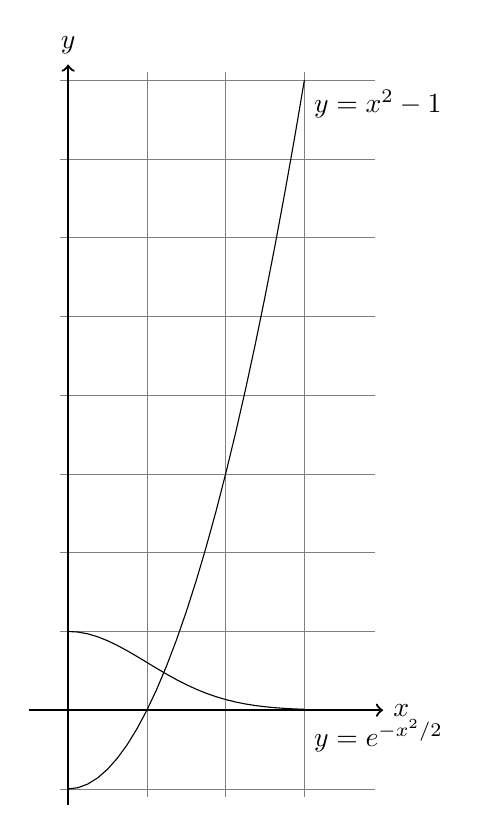
\begin{tikzpicture}
\draw[very thin,color=gray] (-0.1,-1.1) grid (3.9,8.1);
\draw[->,thick] (-0.5,0) -- (4,0) node[right] {$x$};
\draw[->,thick] (0,-1.2) -- (0,8.2) node[above] {$y$};

\draw[domain=0:3] plot (\x,{\x*\x-1}) node[below right] {$y = x^2-1$};
\draw[domain=0:3] plot (\x,{exp(-\x*\x/2)}) node[below right] {$y = e^{-x^2/2}$};
\end{tikzpicture}
\end{verbatim}

\begin{center}
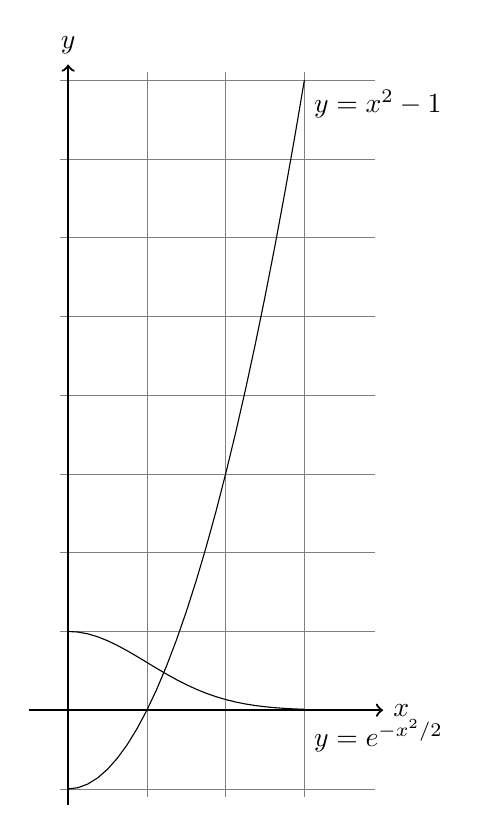
\begin{tikzpicture}
\draw[very thin,color=gray] (-0.1,-1.1) grid (3.9,8.1);
\draw[->,thick] (-0.5,0) -- (4,0) node[right] {$x$};
\draw[->,thick] (0,-1.2) -- (0,8.2) node[above] {$y$};

\draw[domain=0:3] plot (\x,{\x*\x-1}) node[below right] {$y = x^2-1$};
\draw[domain=0:3] plot (\x,{exp(-\x*\x/2)}) node[below right] {$y = e^{-x^2/2}$};
\end{tikzpicture}
\end{center}
重點是
\begin{itemize}
  \item 一樣用中括號設定參數,用 ( ) 設定起始點,終點
  \item 畫格子 grid,除了 grid 還有之前看到的 circle, rectangle...。
  \item node 寫文字, 擺設位置設定在起始點的 below, above, right, left,
    在 pgfplots 裡面用east, south, west, north 東南西北表示。
  \item 用 \verb=->= 畫箭頭
  \item 用 color 畫顏色
  \item 指定線粗細用 thin, thick ...
  \item plot 畫 symbolic 運算
  \item domain 設定 symbolic 運算範圍
\end{itemize}
顏色與粗細設定
\begin{itemize}
  \item black, red, green, blue, cyan, magenta, ...
  \item ultra thin, very thin, thin 三種 thin
  \item ultra thick, very thick, thick 三種 thick
\end{itemize}
\begin{center}
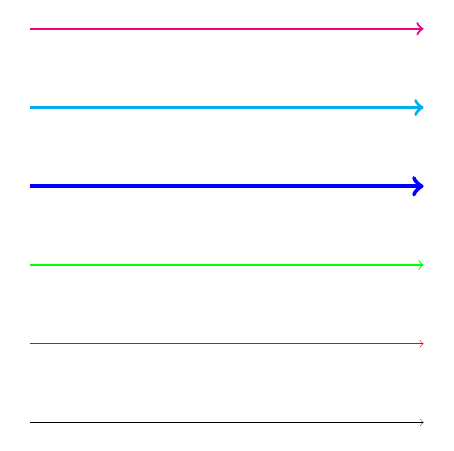
\begin{tikzpicture}
\draw[->,ultra thin, color=black] (0,1) -- (5,1);
\draw[->,very thin,color=red] (0,2) -- (5,2);
\draw[->,thin,color=green] (0,3) -- (5,3);
\draw[->,ultra thick,color=blue] (0,4) -- (5,4);
\draw[->,very thick,color=cyan] (0,5) -- (5,5);
\draw[->,thick,color=magenta] (0,6) -- (5,6);
\end{tikzpicture}
\end{center}
最後 tikzpicture 有很多 library 可以套用,只要用 usetikzlibrary 引用
,例如 patterns 跟 snakes
\begin{verbatim}
\usetikzlibrary{patterns,snakes}

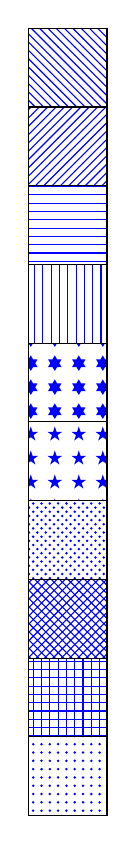
\begin{tikzpicture}
\draw[pattern=dots, pattern color=blue] (0,0) rectangle ++(1,1);
\draw[pattern=grid, pattern color=blue] (0,1) rectangle ++(1,1);
\draw[pattern=crosshatch, pattern color=blue] (0,2) rectangle ++(1,1);
\draw[pattern=crosshatch dots, pattern color=blue] (0,3) rectangle ++(1,1);
\draw[pattern=fivepointed stars, pattern color=blue] (0,4) rectangle ++(1,1);
\draw[pattern=sixpointed stars, pattern color=blue] (0,5) rectangle ++(1,1);
\draw[pattern=vertical lines, pattern color=blue] (0,6) rectangle ++(1,1);
\draw[pattern=horizontal lines, pattern color=blue] (0,7) rectangle ++(1,1);
\draw[pattern=north east lines, pattern color=blue] (0,8) rectangle ++(1,1);
\draw[pattern=north west lines, pattern color=blue] (0,9) rectangle ++(1,1);
\end{tikzpicture}
\end{verbatim}
\begin{center}
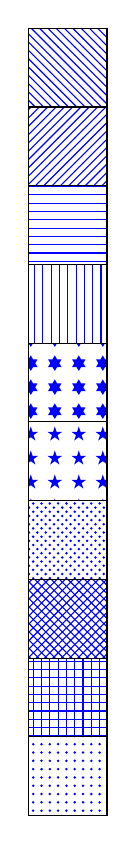
\begin{tikzpicture}
\draw[pattern=dots, pattern color=blue] (0,0) rectangle ++(1,1);
\draw[pattern=grid, pattern color=blue] (0,1) rectangle ++(1,1);
\draw[pattern=crosshatch, pattern color=blue] (0,2) rectangle ++(1,1);
\draw[pattern=crosshatch dots, pattern color=blue] (0,3) rectangle ++(1,1);
\draw[pattern=fivepointed stars, pattern color=blue] (0,4) rectangle ++(1,1);
\draw[pattern=sixpointed stars, pattern color=blue] (0,5) rectangle ++(1,1);
\draw[pattern=vertical lines, pattern color=blue] (0,6) rectangle ++(1,1);
\draw[pattern=horizontal lines, pattern color=blue] (0,7) rectangle ++(1,1);
\draw[pattern=north east lines, pattern color=blue] (0,8) rectangle ++(1,1);
\draw[pattern=north west lines, pattern color=blue] (0,9) rectangle ++(1,1);
\end{tikzpicture}
\end{center}
snakes
\begin{verbatim}
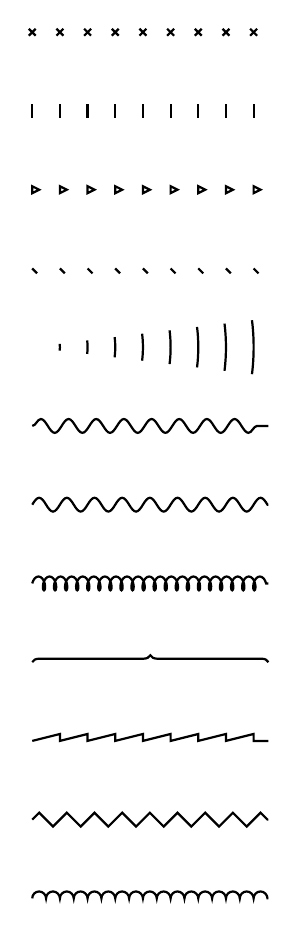
\begin{tikzpicture}[thick]
\draw[snake=bumps] (0,0) -- (3,0);
\draw[snake=zigzag] (0,1)-- (3,1);
\draw[snake=saw] (0,2) -- (3,2);
\draw[snake=brace] (0,3)-- (3,3);
\draw[snake=coil,segment length=4pt] (0,4)-- (3,4);
\draw[snake=coil,segment aspect=0] (0,5) -- (3,5);
\draw[snake=snake] (0,6) -- (3,6);
\draw[snake=expanding waves,segment angle=7] (0,7)-- (3,7);
\draw[snake=border,segment angle=-45] (0,8) -- (3,8);
\draw[snake=triangles] (0,9) -- (3,9);
\draw[snake=ticks] (0,10) -- (3,10);
\draw[snake=crosses] (0,11) -- (3,11);
\end{tikzpicture}
\end{verbatim}
\begin{center}
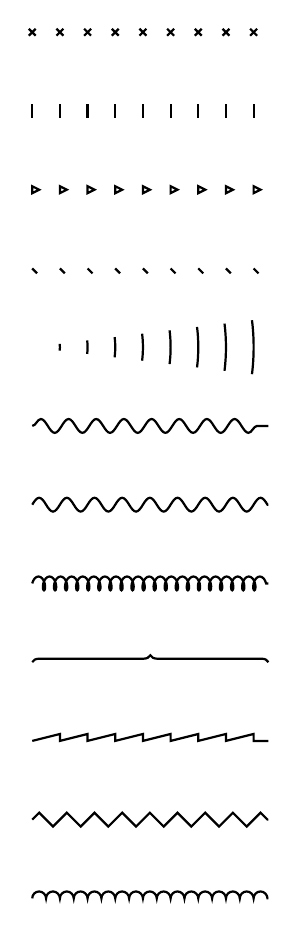
\begin{tikzpicture}[thick]
\draw[snake=bumps] (0,0) -- (3,0);
\draw[snake=zigzag] (0,1)-- (3,1);
\draw[snake=saw] (0,2) -- (3,2);
\draw[snake=brace] (0,3)-- (3,3);
\draw[snake=coil,segment length=4pt] (0,4)-- (3,4);
\draw[snake=coil,segment aspect=0] (0,5) -- (3,5);
\draw[snake=snake] (0,6) -- (3,6);
\draw[snake=expanding waves,segment angle=7] (0,7)-- (3,7);
\draw[snake=border,segment angle=-45] (0,8) -- (3,8);
\draw[snake=triangles] (0,9) -- (3,9);
\draw[snake=ticks] (0,10) -- (3,10);
\draw[snake=crosses] (0,11) -- (3,11);
\end{tikzpicture}
\end{center}
鴨子
\begin{verbatim}
\usetikzlibrary{ducks}


\begin{tikzpicture}
  \draw (0,0) pic[
    duck/water=green,
    duck/alien,
    ] {duck};
  \draw (4,0) pic[
    scale=1.4,
    ] {duck};
\end{tikzpicture}
\end{verbatim}
\begin{center}

\begin{tikzpicture}
  \draw (0,0) pic[
    duck/water=green,
    duck/alien,
    ] {duck};
  \draw (4,0) pic[
    scale=1.4,
    ] {duck};
\end{tikzpicture}
\end{center}
這些工具所畫圖都能跟之前插圖用的 figure, wrapfig 共用,也能用上索引 caption。
\\\\
其實還有很多其他有趣的畫圖工具,有的畫工程圖或 x-y 圖也很漂亮,基本上三種繪圖
工具都非常多設定,所以最後還是要 google 看人家的範例改成自己想要的,無論什麼圖
,大致都能快速精準畫出。

\end{document}
